\chapter{Modulation of sharp-wave incidence}
\label{chap:swr}

\section{Summary}
  Recent \textit{in vitro} studies have demonstrated that sharp-wave ripple
  events can be evoked after optogenetic stimulation of a parvalbumin-positive
  interneuron subpopulation \citep{Schlingloff2014, Kohus2016}. The
  2-population model described in the previous chapter cannot explain this
  phenomenon. In this chapter, a 3-population model is discussed in detail as a
  hypothetical disinhibitory circuit that can generate the population bursts in
  the CA areas of the hippocampus. The main theme addressed here is how the
  GABAergic transmission modulates the incidence of sharp-wave ripple events.
  In particular, it is unknown how gabazine, a $\rm GABA_A$ receptor antagonist,
  suppresses the generation of sharp-wave ripples. Analyzing data from
  \textit{in-vitro} recordings and dissecting the 2-population model \textit{in
  silico} and analytically gives a few possible explanation of the gabazine
  effect. The results are interpreted in the light of the proposed circuit.
  Another question explored here is whether the slow dynamics of $\rm GABA_B$
  receptors is modulating the long time scale of the inter-event intervals,
  that is in the order of hundreds of milliseconds to tens of seconds.

\section{Introduction}
  Sharp-wave ripples (SWRs) are network events in the hippocampus that involve
  large numbers of cells that fire in synchrony within a time window of
  $\sim20-100\, \mathrm ms$ \citep{Buzsaki2015}. During SWRs \textit{in vivo},
  principal neurons can fire in a temporal order that reflects the behaviour
  sequences from previous \citep{Lee2002} or future episodes
  \citep{Dragoi2011}. Such replays are important for the consolidation of newly
  formed memories \citep{Girardeau2009}. Despite the concentrated effort and
  the progress in studying SWRs, some basic understanding of the emergence and
  the development of these events is still lacking. Therefore,
  \textit{in-vitro} models have been developed to facilitate the study of this
  peculiar phenomenon \citep{Maier2003}. In particular, \textit{in-vitro}
  preparations provide a better experimental control over the hippocampal
  circuit generating SWRs, e.g., facilitation of recording and imaging,
  isolation of specific microcircuits, pharmacological manipulation of
  substances, etc.

  In this introduction, I review some general facts from the literature
  concerning the generation of SWRs. Because of the importance of inhibition
  \citep[e.g.,][]{Maier2003, Schlingloff2014}, I start with a brief overview of
  the main characteristics of the GABAergic neurons and the types of synapses
  they form in the hippocampus. In the following I will provide a brief
  discussion on some pharmacological substances that modulate the incidence of
  spontaneous SWRs \textit{in vitro}. The last section of this introduction is
  dedicated to a hypothetical 3-population network model that can explain some
  of the more counterintuitive findings reported in the literature. 
  %Throughout
  %the following text, the terms sharp-wave ripple (SWR) and sharp wave (SW) are
  %used interchangeably referring to the same population event. The cases when
  %the fast ripple oscillations are specifically discussed are mentioned
  %explicitly.

  \subsection{Inhibitory transmission in the hippocampus}
    $\gamma$-Aminobutyric acid (GABA) is the main inhibitory neurotransmitter
    in the central neural system \citep{Sivilotti1991}. GABA is produced by
    inhibitory neurons (INs) and stored in vesicles at the presynaptic
    terminals. GABA is released spontaneously or after a presynaptic neuronal
    action potential (AP). The action of GABA at the synapses is terminated by
    uptake mechanisms from the presynaptic side or from the surrounding glial
    cells. There are two major classes of receptors that are sensitive to the
    released GABA: $\rm GABA_A$ and $\rm GABA_B$ receptors. 

    \subsubsection{$\rm GABA_A$ receptors}
    \label{sec:gabaa}
      %gabaa is ubiquitous sim x\% of all synapses?
      The $\rm GABA_A $ receptor ($\rm GABA_A R$) is a ligand-gated channel
      that selectively conducts chloride ions ($\rm Cl^-$) upon activation by
      agonists such as GABA. Typically, this results in an inhibitory
      postsynaptic potential (IPSP) and the hyperpolarization of the cell
      membrane. The reversal potential of the mediated IPSP is determined by
      the ratio of intracellular and extracellular chloride concentration and
      is typically $\sim -70\, \rm mV$. Inhibitory interneurons target with
      every compartment of the hippocampal principal cells (PCs), and $\rm
      GABA_ARs$ can be found everywhere along the axo-dendritic axis of both
      PCs and INs \citep{Kullmann2005}.
      %ref on nonGABAergic interneurons vida?

      Structurally, $\rm GABA_ARs$ are protein complexes that consist of 5
      subunits arranged in a ring. The subunits form a central pore through
      which chloride ions can flow (Figure~\ref{fig:gabaa}). Multiple possible
      combinations of subunits (an incomplete list is shown in the chart in
      Figure~\ref{fig:gabaa}) can form a receptor. The set of subunit
      determines basic kinetic properties such as activation and deactivation
      time constants \citep{Benkwitz2004, Boileau2005}, and also the affinity
      to GABA, benzodiazepines, steroids, barbiturates, ethanol, etc. The most
      abundant subunit combination is $\alpha_1 \beta_2 \gamma_2$ (shown in
      Figure~\ref{fig:gabaa}C). For example in the hippocampal CA3 area, 90\%
      of the perisomatic synapses on PCs are immunopositive for the $\alpha_1$
      subunit \citep{Kerti2016}. However, not all inhibitory synapses found by
      immunolabeling are active. Some inhibitory synapses might remain silent
      due to the lack of presynaptic GABA \citep{Bekkers2005}. Much like their
      excitatory cousins, the strength of inhibitory synapses is subjected to
      plasticity by various spike-timing-dependent-plasticity (STDP) rules
      \citep[as reviewed by][]{Vogels2013}.

      \begin{figure}
        \center
        \includegraphics[width= 32pc]{gabaa_alpha.png}
        \caption{
          The $\rm GABA_A$ receptor complex.
          {\bf A,} Rotationally averaged representation of electron microscope
          image reveals a fivefold symmetry of the $\rm GABA_AR$
          (\citealp{Nayeem1994}; adapted with permission). The receptor
          diameter is $\sim 10\,\rm nM$.
          {\bf B,} Sketch of the most typical $\rm GABA_AR$ $\alpha_1
          \beta_2 \gamma_2$ with the location of the GABA and benzodiazepines
          (BZD) binding sites (adapted from Wikipedia Commons).
          {\bf C,} Chart showing the approximate distribution of $\rm
          GABA_AR$ according to the subunits expression from a rat brain
          (\citealp{Whiting2003}; adapted with permission).
               }
      \label{fig:gabaa}
      \end{figure}
      
      % tonic
      Not all $\rm GABA_ARs$ are located at the synapses. A major subclass of
      $\rm GABA_ARs$ containing the $\delta$ subunit are located
      extrasynaptically on the membrane of cell bodies or dendrites. These
      receptors are especially sensitive to the ambient GABA that is released
      from presynaptic terminals and diffused from the synaptic cleft into the
      extracellular space \citep{Semyanov2004, Farrant2005}. Their activation
      leads to a ``tonic'' hyperpolarization of the cell membrane, which
      contrasts the rapid dynamics of phasic IPSPs. Tonic $\rm GABA_A Rs$
      express a wide range of modulations. Their activity depends on the amount
      of GABA released from the nearby located synapses, and by the changes in
      GABA uptake \citep{Farrant2005}.

    \subsubsection{$\rm GABA_B$ receptors}
      $\rm GABA_B$ receptors ($\rm GABA_BRs$) are another major class of
      inhibitory GABAergic receptors that are expressed in most neurons of the
      central nervous system \citep{Gassmann2012}. They are metabotropic
      receptors, that is, acting through G~proteins. A functional $\rm
      GABA_BR$ consists of two subunits: $\rm GABA_{B1a}$ or $\rm GABA_{B1a}$,
      and $\rm GABA_{B2}$. The $\rm GABA_BRs$ can be located at the post- or
      presynaptic side of the terminals.  Postsynaptic $\rm GABA_BRs$ are
      located near the glutamatergic synapses but not at the inhibitory ones.
      There, they activate the G-protein-activated inwardly rectifying
      potassium channels (GIRKs) that inhibit the neuronal activity by
      generating a slow IPSP ($\sim 500 \rm \, ms$) with a low reversal
      potential of $\sim - 100\, \rm mV$ \citep{Booker2013}. The postsynaptic
      receptor activation is considered important in the modulation of the
      long-term synaptic plasticity by controlling the backpropagation of APs
      \citep{Leung2006}. Presynaptic $\rm GABA_BRs$ can be located at
      excitatory or inhibitory terminals, acting as hetero- or autoreceptors,
      respectively. Activation of the presynaptic $\rm GABA_BRs$ reduces the
      permeability of the voltage-gated $\rm Ca^{2+}$ channels (VGCCs)
      resulting in inhibition of $\rm Ca^{2+}$ influx at the terminal, and
      thus, in reduction of the evoked and spontaneous neurotransmitter release
      \citep{Gekel2008}. Autoreceptors can be activated by a single AP of the
      cell they are located on \citep{Kobayashi2012}, while postsynaptic
      activation requires repetitive GABAergic firing \citep{Scanziani2000}.

      In the hippocampus, the $\rm GABA_BRs$ are differentially expressed
      across the hippocampal layers and across neural populations.
      Postsynaptic, GIRK-coupled receptors are expressed over the whole
      somato-dendritic axis of the hippocampal principal cells, with the
      highest densities in the radiatum and in the distal dendrites in stratum
      lacunosum-moleculare in the CA regions \citep{Degro2015}. Compared to CA1
      and dentate gyrus, pyramidal cells in area CA3 exhibit substantially
      stronger IPSPs induced by the $\rm GABA_BR$ agonist baclofen
      \citep{Degro2015}.  Interneurons show population-specific expression of
      postsynaptic $\rm GABA_BRs$. For example, immunolabeling reveals high
      $\rm GABA_{B1}$ subunit density at the extrasynaptic membrane of PVBC. In
      response to an extracellular stimulation in CA1, parvalbumin positive
      ($\rm PV^+$) basket cells have larger $\rm GABA_B$-mediated IPSCs
      compared to the ones evoked in the dendritic-targeting $\rm PV^+$
      interneurons \citep{Lei2003}. Synaptic transmission from both
      glutamatergic and GABAergic synapses on interneurons in the
      stratum radiatum is inhibited by $\rm GABA_BR$ activation. Moreover, $\rm
      GABA_BR$ activation reduces the frequency-dependent and short-term
      depression of inhibitory transmission and normalizes the IPSPs on
      principal cells. $\rm PV^+$ dendritic-targeting interneurons show higher
      densities of $\rm GABA_BRs$ in the axons compared to $\rm PV^+$ basket
      cells \citep{Booker2013}.

  \subsection{GABAergic modulation of sharp-wave ripple incidence \textit{in vitro}}
  \label{swr_modulation}
    \textit{In-vitro} slice preparations are ideally suited to study the local
    hippocampal circuitry. Under certain experimental conditions, slices can
    express spontaneous events that resemble the SWRs observed \textit{in vivo}
    \citep{Hajos2009, Maier2009}. These results suggest that a fraction of the
    hippocampal circuitry is sufficient for the generation of SWRs.
    \textit{In-vitro} preparations have a slice thickness typically $\sim 500
    \, \rm \mu m$, containing $\sim$ 20,000--40,000 neurons in the CA areas
    \citep[an estimate based on the numbers of neurons in the rat hippocampus
    and slice thickness;][]{Boss1985, West1991, Bezaire2013}. Moreover,
    mini-slice experiments show that isolated CA3 and CA1 areas can also
    generate SWRs in the absence of connections to neighboring regions
    \citep{Maier2003}. Despite the relatively small network size, the dynamics
    of the hippocampal circuit is not well understood, and a complete model of
    the SWR generation mechanism is still missing.

    Because of the larger neuronal excitability of the ventral parts of the
    hippocampi \citep{Dougherty2012}, SWRs \textit{in-vitro} models usually
    rely on ventral slices \citep[e.g.,][]{Maier2003, Nimmrich2005}. SWRs
    normally originate spontaneously in the CA3 region with a stereotypical
    waveform shape consisting of the sharp wave and the ripple oscillation in
    the field potential \citep{Csicsvari1999}. The activity then propagates to
    the CA1 area via the Schaffer collateral pathway. The ripples are, however,
    incoherent in both regions, suggesting an independent origin of the fast
    oscillation \citep{Csicsvari2000, Both2008}. The \textit{in-vitro} model
    provides the opportunity of experimental control, and thus, to disentangle
    the contribution of various factors such as the contribution of different
    neuronal populations, neurotransmitter signalling, etc.
    
    Inhibitory transmission plays a central role in the generation of SWRs
    \citep{Maier2003, Schlingloff2014}. Drugs altering the properties of
    inhibitory transmission can shed light on the different signaling paths
    involved the generation of SWRs. For example, SR-95531 (gabazine) is a
    widely used $\rm GABA_A$ antagonist that has high affinity to the GABA
    binding site of phasic receptors \citep{Ueno1997, Bai2001, Yeung2003}.  Low
    doses of gabazine \textit{in vitro} decrease the incidence of SWRs, while
    larger doses block the events \citep{Maier2003, Nimmrich2005,
    Ellender2010}. Currently, it is unclear through what mechanisms gabazine
    affects the SWR incidence.
    %It is been shown that bicuculline, another $\rm GABA_A$ antagonist also
    %decreases the SWR incidence \textit{in vivo} \citep{Suzuki1988}, however up
    %to my knowledge, its effect \textit{in vitro} is not known.
    On the other hand, thiopental is a barbiturate that increases the IPSP
    decay time constant, and thus, increases the total charge at the
    postsynaptic side \citep{Dickinson2002}.
    %At higher concentrations it activates also the tonic $\rm GABA_A Rs$.
    Low doses of thiopental decrease SWR incidence, while prolonging the
    duration and the peak of the spontaneous events, and interestingly, reduce
    the number of ripples per event \citep{Papatheodoropoulos2007}. Moreover,
    how can two drugs (i.e., gabazine and thiopental) that have opposite
    effects on the GABA synapses affect SWRs in a similar manner, i.e.,
    decreasing the incidence of spontaneous SWRs?

    Other major drugs affecting $\rm GABA_A Rs$ such as diazepam and
    phenobarbital have nonlinear effects on SWR incidence: for low doses
    the occurrence is increased, and for higher concentrations the incidence
    goes down \citep{Papatheodoropoulos2007, Koniaris2011}. These effects are
    not well understood.
  
    %GB: 
    The role in the modulation of SWRs of the other major inhibitory receptor,
    the $\rm GABA_B R$ is unclear. Some studies have reported that blocking
    $\rm GABA_B Rs$ in slices doesn't alter the SWR properties, such as
    incidence, amplitude, duration \citep{Hollnagel2014, Hofer2015}. However,
    later in this chapter I will show that in the \textit{in-vitro} model
    analysed here, the $\rm GABA_B Rs$ antagonist SCH50,911 increases the
    incidence of SWRs. Blocking the GIRK channels with SCH23,390 also results
    in an increase of SWR incidence (\citealp{Maier2012}; personal communication
    with Nikolaus Maier). On the other hand, the application of $\rm GABA_B R$
    agonists decreases the incidence of SWR events \citep{Maier2012,
    Hollnagel2014}.

    %here I answer some of these questions, others are left as open.

  \subsection{Sharp-wave events driven by inhibition}
    A counterintuitive experimental finding is the fact that SWRs can be evoked
    by driving inhibitory neurons to fire \citep{Ellender2010, Schlingloff2014,
    Kohus2016}. In particular, \cite{Schlingloff2014} have demonstrated that
    SWRs can be elicited by a transient optogenetic drive of a subpopulation of
    parvalbumin-positive ($\rm PV^+$) interneurons
    (Figure~\ref{fig:Schlingloff6}). The authors show that SWRs are evoked a
    few milliseconds after the onset of the light stimulation, and that the
    number of ripples is stable irrespective of the length of the impulse
    (Figure~\ref{fig:Schlingloff6}E). Spontaneous SWRs do not occur when
    ionotropic excitatory transmission is blocked, but nevertheless, events can
    be evoked by optogenetic stimulation of a $\rm PV^+$ subpopulation. This
    finding suggests that inhibitory activity is sufficient for the generation
    of SWRs in the pyramidal layer, given that there is appropriate drive for
    the circuit, e.g., optical stimulation with duration of $\sim 20 \, \rm
    ms$. In the control condition, when no synapses are blocked, the $\rm PV^+$
    stimulation recruits excitation. During the evoked SWRs, whole-cell
    voltage-clamp recordings from $\rm PV^+$ interneurons reveal phasic
    excitatory postsynaptic potentials (Figure~\ref{fig:Schlingloff79}),
    meaning that the inhibitory stimulation leads to the release of excitation.

    \begin{figure}
      \center
      \includegraphics[width= 25pc]{Schlingloff_f6.png}
      \caption{
        Sharp-wave ripples can be evoked by optogenetic drive to $\rm PV^+$ interneurons
        (\citealp{Schlingloff2014}; adapted with permission)
        {\bf A,} Fluorescent staining against parvalbumin (red) and ChR2
        (green) shows that ChR2 is expressed exclusively in $\rm PV^+$
        interneurons. str. o., stratum oriens; str. rad., stratum radiatum;
        str. pyr., stratum pyramidale.
        {\bf B,} Spontaneous and light-evoked (blue bars) SWRs recorded from a
        slice in control conditions. Spontaneous events disappear after a
        blockage of excitatory ionotropic transmission (red bar). 
        {\bf C,} A zoom in the local field potential from the periods denoted
        with 1 and 2 in \textbf{B}. Spontaneous events are denoted with stars,
        evoked events are denoted with a blue bar indicating the timing of the
        light pulse. During the excitatory blockage no spontaneous SWRs occur,
        but only evoked (right panel).
        {\bf D,} Examples of a spontaneous SWR (left), an evoked SWR (right),
        and an evoked SWRs with excitation blocked.
        {\bf E, F,} Light pulses with different durations evoke SWRs. In
        control condition, the length of the SWR event is relatively independent
        on the light duration, which is not the case when excitation is blocked.
             }
    \label{fig:Schlingloff6}
    \end{figure}

    How does the $\rm PV^+$ interneurons population lead to the excitatory
    drive observed in the {\it in-vitro} model? A simple two-population model
    consisting of single excitatory and inhibitory populations cannot explain
    the above-mentioned phenomenon. To better understand the mechanisms behind
    SWR generation one needs to look beyond the 2-population model (as
    presented in Chapter~\ref{chap:asss}) and consider additional
    mechanisms. A few explanation have been proposed in the literature:
    \begin{enumerate}
      \item \textbf{Depolarizing effects of $\rm GABA_ARs$.} It has been shown
        that during the early phases of development and during certain
        conditions of {\it in-vitro} preparations $\rm GABA_ARs$ can have
        depolarizing effects on the postsynaptic membrane potentials of
        pyramidal cells \citep{Cohen2002, Gulledge2003, Banke2006}. In
        particular, \cite{Szabadics2006} demonstrated how activation of a
        single axo-axonic cell can trigger a depolarizing GABAergic
        postsynaptic potential or a postsynaptic action potential in pyramidal
        cell in cortical slices from rats and humans. In such a scenario,
        driving the $\rm PV^+$ interneuron population (that includes the
        axo-axonic cells) would have an excitatory effect on the network
        activity.
      \item \textbf{Inhibition leads to rebound excitation.} \cite{Cobb1995}
        have shown that inhibitory inputs to depolarized pyramidal neurons can
        lead to a brief depolarization (rebound) following the initial
        hyperpolarization. During the rebound depolarization cells can fire
        action potentials. Such effects taking place simultaneously in multiple
        neurons would effectively lead to their transient synchronization, and
        thus, to a possible population burst.
      \item \textbf{Inhibition de-inactivates voltage-gated ion channels.} This
        idea is in line with \cite{Platkiewicz2011} who have shown that the
        inactivation of $\rm Na^+$ channels impacts the neuron's firing
        threshold. A brief inhibitory/hyperpolarizing input might be sufficient
        to de-inactivate channels that have been inactivated due to continuous
        depolarization. This mechanism can be extended also to other
        voltage-gated ion channels. 
      \item \textbf{Disinhibition.} A possible disinhibitory loop includes
        basket cells, which are shown to project to dendritic-targeting
        interneurons (DTIs) \citep{Cobb1997, Kohus2016}. According to this
        hypothesis activation of BC leads to strong inhibition of the DTI that
        actively suppress PC from firing between the events. This inhibition of
        inhibition would be the direct cause of the following SWR.
    \end{enumerate}
    
    \begin{figure}
      \center
      \includegraphics[width= 33pc]{Schlingloff_f79.png}
      \caption{
        Optogenetic control of $\rm PV^+$ interneurons modulates SWRs
        (\citealp{Schlingloff2014}; adapted with permission).
        {\bf A,} Optogenetic drive of $\rm PV^+$ interneurons evoked repetitive action
        potentials in $\rm PV^+$ cells (loose-patch recording in top trace) as well as a
        SWR in the LFP (second trace). A whole-cell, voltage-clamp recording 
        from a $\rm PV^+$ interneuron shows phasic EPSC $<10 \, \rm ms$
        after the onset of the impulse (two bottom traces).
        \textbf{B,} Optogenetic silencing of $\rm PV^+$ cells interrupts (left
        panel) and blocks the generation of spontaneous SWRs (right panel).
             }
    \label{fig:Schlingloff79}
    \end{figure}

    The above-mentioned mechanisms are not mutually exclusive as possible
    causes for the inhibitory-driven evoked events. However, some of these
    explanations seem more plausible than others. For example, currently there
    is no evidence that $\rm GABA_AR$ has depolarizing effects in the
    \textit{in-vitro} SWR models. Experimental support for membrane potential
    rebounds after inhibitory inputs from PVBCs is also scarce. This hypothesis
    comes with clear predictions that can be tested experimentally
    \textit{in-vitro}: i) a patch-clamped recordings from PC should show a
    rebound spike after driving one or more $\rm PV^+$ interneurons; and ii),
    blocking de-inactivation of the voltage-gated ion channels should prevent
    the inhibitory-driven SWRs. 
    
  \subsection{Hypothesis on the CA3 circuitry giving rise to sharp-wave ripples}
  \label{sec:3pop}

    The fact that silencing a $\rm PV^+$ subpopulation can interrupt an ongoing
    SWR event and significantly reduce the incidence of spontaneously occurring
    events \citep{Schlingloff2014} supports the last hypothetical mechanisms,
    the disinhibitory circuit (Figure~\ref{fig:3pop}). The hypothesis presented
    below aims to explain some paradoxical results reported in the literature.
    The proposed model relies on a number of assumptions that are to be tested
    in experiments. Moreover, it comes with some predictions that can validate
    or invalidate the proposed model.

    \begin{figure}
      \center
      \includegraphics[width= 25pc]{3pop_gamma.png}
      \caption{
        A sketch of a minimal model consisting of 3 neuronal populations.
        \textbf{left:} The network consist of 3 populations: PC
        (right), PVBC (left), and mIN (top). Populations are all-to-all
        connected, including recurrent connections (not shown). Axons and
        synapses are color-coded with red for excitation and blue for
        inhibition.
        \textbf{right:} Population activity before and during a SWR represented
        in three snapshots. The degree of population activation is color-coded
        where higher saturation of the red color denotes higher activity. In
        the background state, PCs and PVBCs have low firing rates, while the
        mIN population has its highest activity. At the onset of events, PCs
        and PVBCs are active, while mINs are silent because of the fast
        inhibition from PVBC. Towards the end of the event, mINs get activated
        by the excitatory neurons, and thus, start suppressing the SWR event.
             }
      \label{fig:3pop}
    \end{figure}
    
    A minimal disinhibitory model consists of 3 populations: pyramidal cells
    (PC), parvalbumin-positive basket cells (PVBC), and another class of
    interneurons, which I will refer to as mysterious interneurons (mINs). The
    circuit can operate in two regimes: a balanced state with low firing rates
    that describes the CA3 network dynamics between events, and a high-firing
    state corresponding to a SWR event (Figure~\ref{fig:3pop}). In the
    background state the PCs are in a low-firing \citep{Csicsvari1999} balanced
    state and are heavily inhibited by the active mINs. The PVBCs are virtually
    silent in the background state \citep{Klausberger2003, Varga2012}.
    Spontaneous SWRs occur when, due to a build-up of activity, pyramidal
    neurons excite the PVBCs, and then PVBCs inhibit the mIN population,
    effectively disinhibiting the pyramidal population. Thus, during a SWR
    event, the network activity turns around, the PC and PVBC populations are
    firing with high rates \citep{Klausberger2003, Varga2012}, while the mINs
    are silent. The conditions in which this disinhibitory circuit operates are
    explored in detail in a separate project by Roberta Evangelista.
    Preliminary results predict a strong PC-PVBC-mIN connection pathway in
    comparison to PC-mIN connections, as well as stronger connections on the
    PVBC-mIN-PC pathway in comparison to PVBC-PC connections.
    
    According to the model, activation of the PC or PVBC population would
    activate the disinhibitory pathway, leading to a SWR. The model is in line
    with the reports that find a gradual build-up of PC activity tens of
    milliseconds prior to spontaneous SWR events \citep{Ellender2010,
    Schlingloff2014, Hulse2016}. Moreover, depolarization of a small group (few
    tens up to hundred) of neighboring pyramidal neurons could evoke a SWR
    \textit{in vivo} \citep{Stark2014}. And \cite{Bazelot2016} showed that
    driving a single pyramidal cell to firing ($200\, \rm pA$, for $200\, \rm
    ms$) can prime the occurrence of SWRs \textit{in vitro}. Interestingly, the
    PC stimulation leads to the recruitment of perisomatic-targeting inhibitory
    interneurons reflected in the field IPSP at the initial phase of the evoked
    SWs. According to the proposed hypothesis, the stimulated PCs
    \citep{Stark2014, Bazelot2016} drive a subpopulation of PVBCs that
    consequently disinhibit the local circuit. Also in line with the
    disinhibitory model is the fact that silencing $\rm PV^+$ cells stops an
    ongoing SWR and leads to suppression of spontaneous SWs
    \citep{Schlingloff2014}.

    %ledri: in vitro epilepsy hippocampal model, activation of a large and diverse IN population
    %leads to a transient epileptyform activity followed by silent period during the continious stimuklation
    %just after the offset of stim, new bursts occur
    The 3-population model is not fully in line with who \cite{Ellender2010}
    have shown that during a continuous ($500\, \rm ms)$ drive of a single
    perisomatic-targeting interneuron, the incidence of SWR occurrence
    decreases, and after termination of the stimulation, the SWR incidence
    increases with a significant peak of occurrence 1 to $2\,\rm seconds$ after
    the stimulation offset. It is worth noting that these results hold only for
    a fraction of the stimulated cells (6/24). Perisomatic-targeting
    interneurons are a family of different classes of interneurons that include
    cholecystokinin-positive basket cells, parvalbumin-positive basket cells,
    and axo-axonic cells \citep{Freund1996}. It is not known which, if any
    particular, class of these interneurons is involved in this temporal
    suppression of SWRs. It is still an open question why stimulating a single
    perisomatic-targeting neuron can suppress SWRs and can release SWRs immediately
    after the stimulation \citep{Ellender2010}, while optical stimulation of small populations
    gives rise to SWRs just $\sim 1\, \rm ms$ after the onset of the
    stimulation \citep{Schlingloff2014}. However, exciting a small
    subpopulation of $\rm PV^+$ interneurons (<5 cells) does not evoke any SWR
    events, and even suppresses ongoing events \textit{in vivo}
    \citep{Stark2014}. This might be explained by the fact that while
    \cite{Schlingloff2014} illuminate the whole slice, and thus activate most
    of the $\rm PV^+$ interneurons, \cite{Ellender2010} and \cite{Stark2014}
    activate one or a very few neurons which is not sufficient for
    disinhibition, and thus, to initiate an event. Another interesting
    disagreement of results is that \cite{Ellender2010} did not observe a rise
    of the SWR incidence after driving single pyramidal neurons in contrast to
    the report from \cite{Bazelot2016}.
    
    To make a more complete model of the SWR generation, one should also
    consider mechanisms that control the duration of a SWR and the time
    interval between events. One requires processes on a relevant time scale on
    the order of hundreds of milliseconds to seconds. An important component of
    such mechanisms could be the short-term plasticity of inhibitory
    transmission. It has been shown that basket cells exhibit short-term
    depression (STD) of synaptic transmission both on pyramidal cells and on
    other interneurons as well \citep{Kraushaar2000, Kohus2016}. During a SWR
    event, PVBCs fire multiple times with a high frequency, and therefore, the
    efficacies of their synapses decrease significantly towards the end of an
    event. Considering such depression on the PVBC-mIN synapses would lead to a
    weaker inhibition on the mINs in the advanced phase of the sharp wave,
    resulting in mINs recruitment. Once active again, mINs inhibit the PC
    population, leading to the termination of the SWR. The recovery of the
    PVBCs synapses is a relatively slow process on the order of hundreds of
    milliseconds \citep{Kohus2016}. Once the synapses recover from depression,
    the PVBC population is able to disinhibit the CA3 circuit again and lead to
    the next event. In line with the STD hypothesis, a prolonged optogenetic
    drive ($400\,\rm ms$) to the PC population leads to ripple oscillations
    that decrease in amplitude and frequency after $50\, \rm ms$
    \citep{Stark2014}. The decrease in frequency is likely due to the
    depression of the PVBC-PVBC synapses that are crucial for the ripple
    oscillation generation \citep{Donoso2017}, while the amplitude decrease is
    due to the depression of PVBC-PC synapses that are the main contributor to
    the ripple LFP in the pyramidal cell layer.

    To summarize, here I propose a phenomenological three-population model as a
    minimal circuit that can give rise to the SWR events observed \textit{in
    vitro} and \textit{in vivo} (see Figure~\ref{fig:3pop}). In the background
    state, in the intervals between events, the pyramidal cell (PC) and the
    $\rm PV^+$ basket cell (PVBC) population exhibit low firing rates, while
    being inhibited by another (not identified yet) inhibitory population
    (mINs). Before the onset of an event, there is a build-up of excitatory
    activity recruiting PVBCs which inhibit the mIN population, and thus, the
    disinhibited circuit enters a high firing-rate regime, where the balance of
    activity is maintained by the pyramidal cells and the PVBCs. The high
    firing rates of PVBCs during the event leads to short-term depression of
    their efferent synapses. In particular, as the PVBC-mIN pathway is
    depressed, the mINs are recruited back into the network, and thus,
    terminate the event by inhibiting the excitatory PC population. 

    Such a model circuit comes with a number of assumptions/predictions that can
    be tested experimentally. A basic model requirement is the third population
    of unidentified interneurons, the mINs. To help narrow down the search for
    this population, there are a few features that should be exhibited
    according to the model:

    \begin{itemize}
      \item mINs are active in the low-firing background state, are silent in
        the initial stage of the SWR events, and are active again at the
        advanced phase of the SWRs. Possible candidates are ivy cells
        \citep{Hajos2013}, axo-axonic cells \citep{Viney2013},
        enkephalin-expressing interneurons \citep{Fuentealba2008b}, or
        neurogliaform cells \citep{Karayannis2010}. However, neurogliaform
        cells and ivy cells have bigger time constants \citep{Fuentealba2008,
        Karayannis2010}, and their slow IPSPs are unlikely to modulate the
        network activity on a millisecond time scale upon $\rm PV^+$
        interneuron stimulation.
      \item a transient inhibition applied to the mIN population should trigger
        a SWR event.
      \item a constant drive applied to the mINs should suppress the generation
        of SWRs.
      \item the mINs are parvalbumin negative ($\rm PV^-$) interneurons.
      \item the mINs are heavily suppressed by a $\rm PV^+$ subpopulation during
        SWR events.
      \item due to the lack of observed IPSPs in patch-clamped pyramidal cell
        recordings, it's likely that mINs target the distal dendrites of PCs.
      \item a current-source density (CSD) analysis from multi-electrode
        recordings might show the location the current source evoked by mINs in
        the background state.
    \end{itemize} 

    However, the proposed disinhibitory hypothesis has to deal with a few
    weaknesses at its incarnation. The following issues need to be addressed
    properly by experiments or extension of the model:

    \begin{itemize}
      \item A light stimulation to the $\rm PV^+$ neurons recruits the
        excitatory population shortly ($\sim 10\, \rm ms$) after the onset of
        the light impulse (see Figure~\ref{fig:Schlingloff79}). This result
        suggests that the membranes of pyramidal cells are in a tight balance
        of excitatory and inhibitory inputs, and the suppression of mINs leads
        to a rapid increase of firing. An interesting question is: Where does
        the excitatory drive originate? In what conditions is the low firing
        rate of the \textit{in-vitro} circuit sufficiently high to drive the
        population bursts upon disinhibition?
         %ref to some measures from PC membranes? hajos?
      \item As mentioned above, patch-clamp recordings from pyramidal cells
        rarely show signatures of IPSPs (from the data provided by Nikolaus
        Maier, and also in \cite{Maier2011, Schlingloff2014}). Assuming that
        the lack of IPSPs is due to a filtering of the dendritic tree, in which
        conditions can this filtering happen?
      \item Given the aforementioned points, it is possible that other
        mechanisms can take the role of the mINs? For example, an alternative,
        or complementary, mechanism to the disinhibition circuit could manifest
        itself though inhibition that would de-inactivate voltage-gated $\rm
        Na^+$ channels.
    \end{itemize}

    In the following Results section, I discuss the findings from \textit{in-vitro} data 
    in the light of the phenomenological model presented here. 

\section{Results}
\label{sec:results}
%________________
  In this section I analyse \textit{in-vitro} recordings provided by Nikolaus
  Maier. All recordings are performed in CA3 stratum pyramidale of hippocampal
  slices that exhibit spontaneous SWRs. The results are interpreted in the
  light of the hypothetical 3-population circuit. Additionally, for explaining
  the experimental findings of gabazine effects in the SWR incidence, I used
  numerical and analytical methods applied to the 2-population network
  presented in Chapter~\ref{chap:asss}.
 
  \subsection{Serial correlations between peak amplitudes of SWRs and intervals between them}
    \label{sec:swr_amp-int}
    The time intervals between consecutive SWR events \textit{in vitro} vary from
    tens of milliseconds to tens of seconds depending on the experimental setup
    and the slice preparation. Currently, we do not know the underlying
    biological processes that control the dynamics on time scales much larger
    than tens of milliseconds. However, a natural assumption is that there is
    some kind of slow recovery of the system after each SWR event, which might
    have been caused by e.g., depletion of synaptic and neuronal resources
    \citep{Cohen2004, Jones2007}, receptor saturation \citep{Trussell1993}, or
    short-term depression \citep{Romani2015, Kohus2016}. Moreover, slow
    dynamics can arise from a slower inhibition evoked by ambient GABA on the
    extrasynaptic $\rm GABA_ARs$ \citep{Brown1978, Ben1994} or an activation of
    synaptic/extrasynaptic $\rm GABA_BRs$ \citep{Scanziani2000, Hollnagel2014,
    Lang2014}. 
  
    The type of data that is analysed here (extracellular recording at a single
    location) does not allow to discriminate between the mechanisms listed
    above as they all predict serial correlations between SWR events. For
    example, if some of the mechanisms is involved indeed, then after a longer
    interval since the last event, the circuit will be more recovered, and the
    following SWR event is expected to be larger in amplitude (see sketch in
    Figure~\ref{fig:sc}, top panel). Moreover, if the SWR peak amplitude
    reflects the degree to which the (local) circuit is involved into the
    population burst, then events with larger amplitudes will cause stronger
    activation of these mechanisms, and thus, a longer interval until the
    following event is expected. To test whether any of the arguments above
    hold, this section examines the serial correlations between
    inter-SWR-interval and the amplitude peak of the following SWR
    (interval-peak), and also the serial correlations between SWR amplitudes
    peaks and the following time interval (peak-interval).

    \begin{figure}
      \centering
      \includegraphics[width= 35pc]{SC.png}
      \caption{Serial correlations of sharp-wave ripples.
        \textbf{top:} An example of extracellular recording. Black and red lines
        are the raw and the band-pass filtered (3--50 Hz) LFP signal,
        respectively. The colored panel below shows the respective spectrogram.
        \textbf{middle:} Typical examples of interval-peak (left panel, $n=294$) and peak-interval
        (right panel, $n=1118$) relations from two different recordings show positive
        correlations. Note the order of magnitude difference in the SWR peak
        amplitude in both examples.
        \textbf{bottom}: Distribution of interval-peak (right panel) and
        peak-interval (left panel) correlations in respect to the SWR
        incidence; the red circles denote significant ($p<10^{-3}$)
        correlations, blue dots denote insignificant correlations.
             }
      \label{fig:sc}
    \end{figure}
  
    Does the recovery time affects the size of the following events? To test
    this, I calculated the serial correlation between the inter-event time
    intervals and the peak amplitude of the following SWR (typical example
    recording shown in Figure~\ref{fig:sc}, middle-left panel). Most slices
    show significant and positive correlations ($p<10^{-3}$; 18 out of 20
    recordings; Figure~\ref{fig:sc}, bottom-left panel). This means that after
    a long interval the amplitude peak of the following SWR is big, and after a
    brief interval, the following SWR has a smaller peak amplitude. After
    dividing the recordings into 5-minute time windows, each slice shows at
    least once positive and significant serial correlation (interval-peak)
    during the course of the recording. Negative correlations are not present.
    The found interval-peak correlations found in the data have been recently
    confirmed by \cite{Kohus2016}.

    In the analysed data, the incidence of spontaneous SWs ranges from 0.1 to
    $\sim 1.2 \,\rm event/sec$ across slices. The degree of recovery might be
    pronounced better for shorter intervals and less pronounced after longer
    intervals. Therefore, a natural question is whether the incidence
    influences the interval-peak correlation. Statistical tests on the
    aggregated data (Figure~\ref{fig:sc}, bottom-left panel) show that this
    dependence is, however, statistically insignificant (r=0.2, p=0.4). Moreover,
    dividing each recording into 5-minute time windows, and testing the serial
    correlation of events within that window in respect to the incidence also
    does not show a strong relation (18 out of 20 recordings show insignificant
    ($p>10^{-3}$), 1/20 positive ($r=0.77 ,\, p<10^{-6}$), and 1/20 negative
    ($r=0.93,\,p<10^{-6}$) correlation between incidence and interval-peak
    correlations). Therefore, the conclusion is that the interval-peak serial
    correlation does not depend on the incidence of SWR events.

    %%%%%%%%%%%%%%%%%%%%%%%%%%%%%%%%%%%%%%%%%%%%%%%%%%%%%%%%%%%%%%%%%%%%%%%%%%%

    Does the SWR peak amplitude influence the time interval until the following
    events? To test that, the peak-interval serial correlation are calculated.
    From 20 slices, only 9 show correlations that are significant
    ($p<10^{-3}$) with a median correlation coefficient of around 0.2
    (Figure~\ref{fig:sc}, bottom-right panel).
    
    % new paragr for locality, new subsection?
    The majority of recordings shows a missing peak-interval correlation
    (11/20). Even though recovery might control inter-SWR intervals, a low
    peak-interval correlation cannot rule out this mechanism. A possible
    explanation for this observation is that the SWR peaks are a local
    phenomenon, and while being large at the recording location, SWs peaks can
    be smaller at other locations of the slice. The next event is then
    triggered in a site where the peak has been rather low and the local
    resources are less depleted. Therefore, we can not predict the time of the
    next event based on the measured amplitude at a particular site because SWs
    can originate elsewhere in the slice. In such cases, the local depletion
    recovery does not play a role in controlling the timing of next events.
    Following this line of reasoning gives us a hypothetical explanation about
    the surprisingly low correlations between peaks and intervals.

    To test the hypothesis relying on the locality of SWR peak amplitudes
    stated above, I analyse data from multi-electrode array (MEA) recordings.
    The dataset is provided by Roberta Evangelista, where multiple sites in the
    CA3 area of hippocampal slices are measured simultaneously. In single
    recordings, the peak amplitudes of SWR events measured at different
    locations show very high co-variability (an example is shown
    Figure~\ref{fig:peak_correlation_ex}). Moreover, the aggregated data from
    20 different slices show that every pair of locations in a CA3 slice has a
    positive and significant ($p<10^{-3}$, 2116 total pairs) correlations between
    the measured SWR peaks (Figure~\ref{fig:peak_correlation_summ}). The high
    correlations between different sites rule out the hypothesis that the
    amplitude of SWRs is a local phenomenon in slices.

    \begin{figure}
      \center
      \includegraphics[width= 35pc]{mea.eps}
      \caption{
        An example multi-electrode array recording {\it in vitro}.
        \textbf{top-left:} A hippocampal slice with recording sites in black.
        The colored circles (red and blue) denote recording channels that are
        considered to be in the stratum pyramidale and have a reliable signal
        of the SWR events. \textbf{bottom:} Example of a recording
        sweep, where SWR peak amplitudes measured 7 recording electrodes are
        plotted in time. For better comparison, peaks are normalized by
        subtracting the mean and dividing by the standard deviation of peaks of
        peak amplitudes for each recording site.  \textbf{top-right:} A matrix
        of the pair-wise correlation coefficients (CC) between SWR peak
        amplitudes measured at the different electrodes.
      }
    \label{fig:peak_correlation_ex}
    \end{figure}

    \begin{figure}
    \centering
      \includegraphics[width= 22pc]{mea_corrs_summ.eps}
      \caption{
        Distribution of correlation coefficients between pairs of SWR peak
        amplitudes measured at different locations in CA3; aggregated data from
        20 hippocampal slices.
             }
    \label{fig:peak_correlation_summ}
    \end{figure}
    
    In summary, the majority of slices (18/20) show positive and significant
    ($p<10^{-3}$) correlations between the time interval since the last event
    and the peak amplitude of the following SWR. On the other hand, smaller
    correlation between SWR peak amplitude and the interval until the
    following event are found in 9/20 slices. This weak peak-interval serial
    correlation can not be explained by some locality of the events as SWR
    peaks are a non-local phenomenon, and a large SWR measured at one location
    is likely to be large in the whole CA3 region.

    The high interval-peak correlations found in the data have been recently
    confirmed by \cite{Kohus2016}. The authors propose that a recovery from
    short-term depression (STD) on the inhibitory synapses affects the
    amplitudes of SWR peaks observed in the local field potential, and
    moreover, suggest that STD is a possible mechanism controlling the SWR
    incidence. The field potential in stratum pyramidale is dominated by the
    inhibitory synaptic activity \citep{Schonberger2014}. Therefore, the
    amplitude of SWR peaks in the stratum pyramidale are modulated by the local
    inhibitory synaptic currents. A recovery from STD of the PVBC-PC synapses
    (and possibly PVBC-PVBC) is a strong candidate for the modulation of SWR
    peak amplitudes. Thus, the high amplitudes of SWRs observed after longer
    time intervals since last event are caused by recovered inhibitory synapses
    in the pyramidal layer. However, the positive peak-interval correlation
    observed in some slices (7/20) suggests that the SWR amplitude might also
    reflect the PVBC firing rate to a smaller degree. In the light of the
    3-population hypothesis stated in Section~\ref{sec:3pop}, the incidence of
    SWRs is controlled by the STD recovery time constant on the inhibitory
    PVBC-mINs synapses, and higher firing PVBC firing would lead to a larger
    depression, and thus, to a longer interval until the next event.

    %parallel recordings of LFP in radiatum can give us an idea about PC activity..

    %power of ripple oscillation might be event better measure for for the recovery after SWR

    %-3 pop: pvbc will affect the depression on pvbc-mins: therefore bigger interrval,
    %and synaptic currents evoked by pvbc are reflected in lfp, but the peak-interval corr
    %is weak; conclussion is taht peaks reflect synaptic currents and to a small degree firing rate...
    %check if there is corrs between peak-interval and incidence...
    
  \subsection{Gabazine effects on sharp-wave ripples {\textit {in vitro}} }
    \label{sec:gabazine_invitro}
    Hippocampal slices exhibit network dynamics shaped by excitatory and
    inhibitory activities that balance each other \citep{Csicsvari1999,
    Maier2011, English2014, Hulse2016}. It is intuitively expected that by
    decreasing the total inhibitory coupling (connections from inhibitory to
    all the other neurons are weakened) the network would get more excitable.
    However, from previous work \citep[e.g.,][]{Nimmrich2005} it is known that
    application of low concentrations of gabazine (a $\rm GABA_AR$ antagonist)
    decreases the rate of spontaneously occurring SWRs, while larger
    concentrations block SWRs \citep{Maier2003, Ellender2010}. It is not clear
    how the application of gabazine affects the network activity. 
    
    An underlying assumption in the presented analysis is that the decrease of
    SWR incidence is due to a decrease of the firing rate of the excitatory
    population outside of SWRs. But how does a decrease of inhibition lead to a
    more inhibited network? To tackle this paradox, in this section I analyse
    some data provided by Nikolaus Maier in which gabazine is applied to
    hippocampal slices.
    
    Gabazine (SR-95531) is a $\rm GABA_AR$ antagonist that binds to the
    GABA-binding site, effectively decreasing inhibitory conductance. Low drug
    concentrations block phasic but not tonic $\rm GABA_ARs$ \citep{Bai2001,
    Yeung2003, Behrens2007}. In the experiments analysed here, after a few
    minutes of stable baseline recording, low concentrations of gabazine ($100
    \,\rm nM$) were applied to the hippocampal slices. A typical example is
    shown in Figure~\ref{fig:gabazine_ex} where gabazine was applied 27 minutes
    after the recording onset (application duration denoted with a horizontal
    red line). Shortly after the drug infusion, the incidence of spontaneous
    events goes down from 0.32 to 0.15 events/second (values are measured in
    5-minute time windows from before and during drug application, independent
    two-sample t-test with p-value $<10^{-6}$). The averaged LFP waveforms
    associated with SWRs (arranged relative to the peak of the filtered signal)
    show a stereotypical SWR waveform before and during the drug application
    (Figure~\ref{fig:gabazine_ex}, bottom panels). There is also slight but
    significant increase of the SWR peak amplitudes and duration after the
    gabazine application ($p<10^{-3}$). After the washout (end of red bar, at
    43 minutes) the incidence of SWs increases back to the values before the
    drug infusion.
    
    \begin{figure}
      \center
      \includegraphics[width =35pc]{6june12_slice1.png}
      \caption{
        An extracellular recording from CA3 where gabazine concentration is
        applied to the hippocampal slice. Time of drug application is denoted
        with a horizontal red bar. The top panel shows the SWR incidence in time
        with a half-minute time resolution. The two panels below show the SWR
        amplitude peaks, where ``fil'' and ``raw'' denote band-passed filtered
        ($\sim 5$--$50\, \rm Hz$, for details see the Methods section) and raw
        voltage traces, respectively; units are in mV. The gray dots represent
        single events, and the black lines represent the mean, and errors bar
        the standard deviation of the amplitude peak in one-minute time
        windows. Analogously, the forth panel shows the SWR duration in
        milliseconds. The panels on the bottom row show all events before,
        during, and after drug application (panels from left to right) overlaid
        in gray, and the mean wave-forms are in black. The right-most panel
        shows a comparison between the mean events from before during, and
        after gabazine application.
      }
      \label{fig:gabazine_ex}
    \end{figure}

    %It is worth noting that in this example recording, there is some
    %high-frequency noise (quantify how high?) in the measured LFP (peaks of the gray traces), likely
    %reflecting the spiking of one or more neurons located nearby the recording
    %electrode. In this example, the network activity seems to be less noisy
    %after the application of gabazine.
    Gabazine decreased the incidence in all 8 slice recordings. In 6 slices the
    decrease was significant ($p<10^{-3}$). The average effect is shown in
    Figure~\ref{fig:gabazine_sum}, where the incidence is normalized (to value
    of 1 for the incidence 5 minutes prior to drug application). Gabazine
    starts affecting the incidence already 1 minute after application and takes
    around 5 minutes to take a full effect. 
    
    \begin{figure}
      \center
      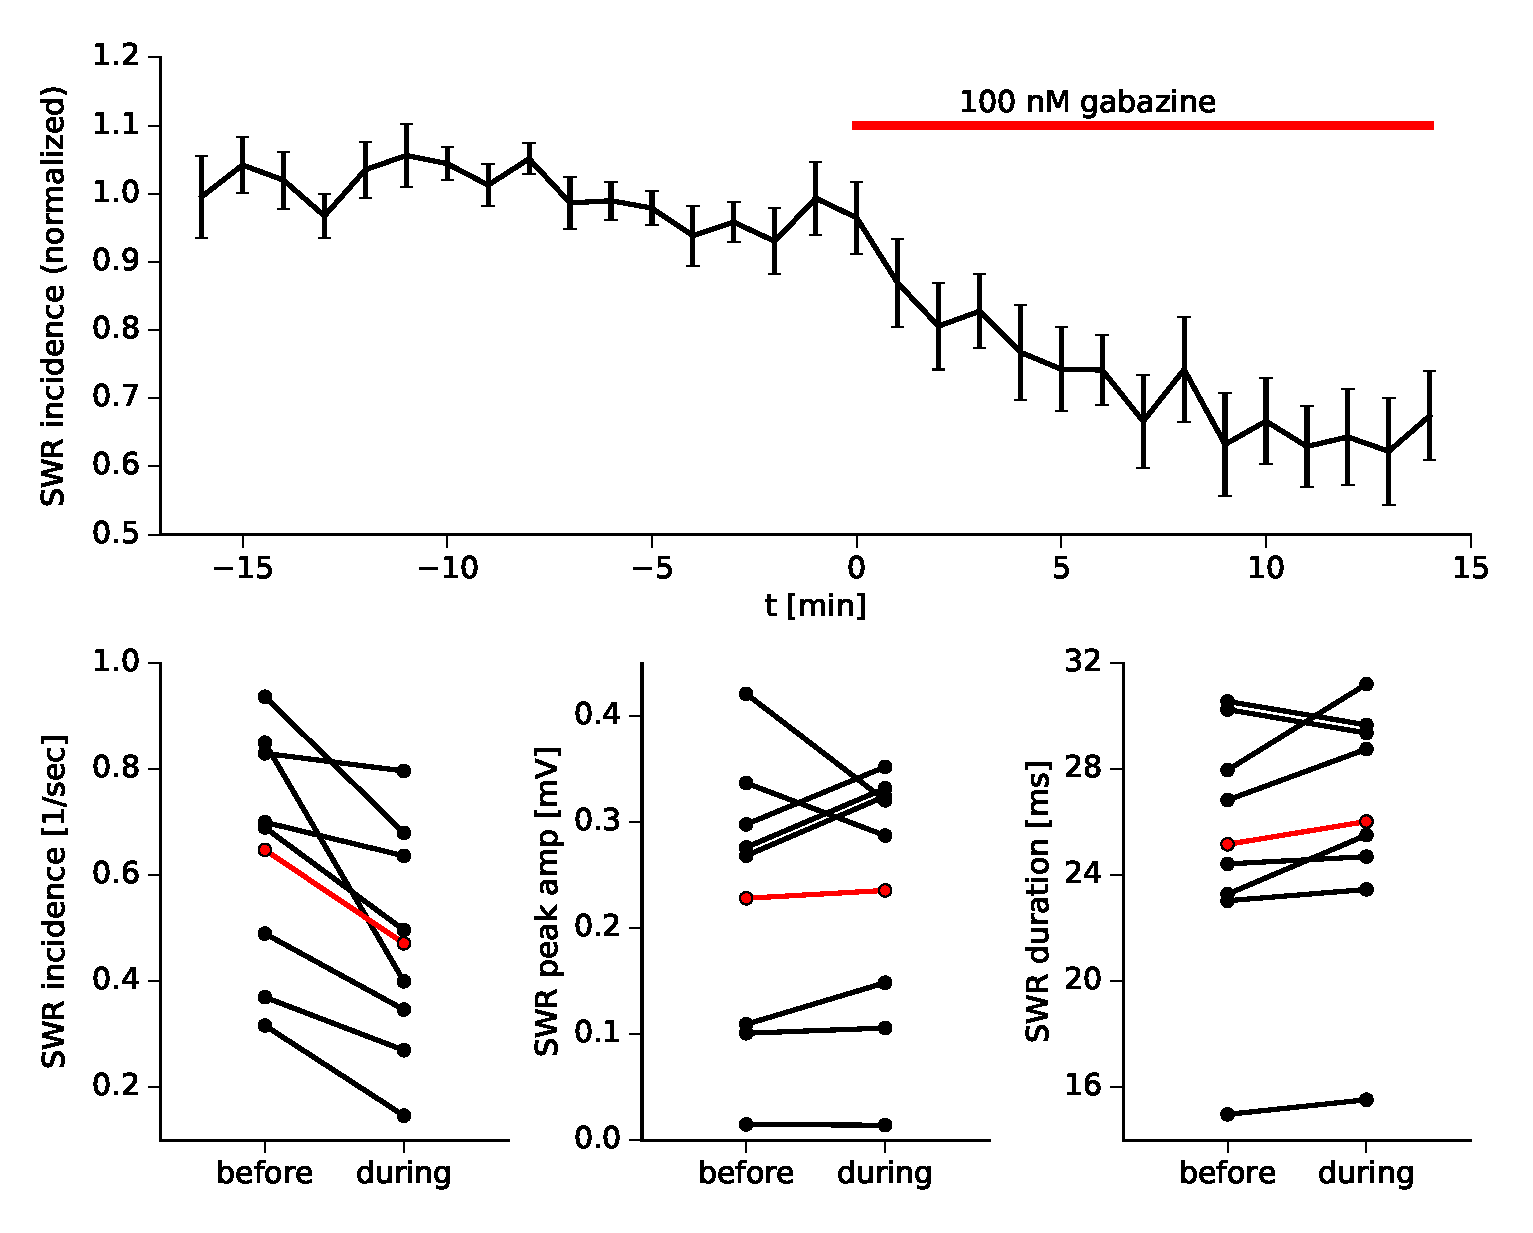
\includegraphics[width =35pc]{gabazine_events_all.eps}
      \caption{
        The $\rm GABA_AR$ antagonist gabazine affects SWRs. {\bf top}: SWR
        incidence in time aggregated from all recordings ($n=8$), where the
        incidence is normalized to 1 by dividing by the mean incidence from
        before the drug application. The red bar shows the time of drug
        application.  {\bf bottom:} The average SWR incidence, peak, and
        duration measured in 5-minute time windows before ([-7, -2] minutes)
        and during ([6, 11] minutes) gabazine application. Each slice is
        denoted with two black dots that are connected by a line. The red dots
        are the averages from all slices.
      }
      \label{fig:gabazine_sum}
    \end{figure}

    To better characterize how the drug affects the network dynamics, the
    further analysis focuses on the events in constrained time windows. Events
    from the window [-7, -2] minutes (before drug application) and [6, 11]
    minutes (after drug application) were used to calculate properties of SWs
    (Figure~\ref{fig:gabazine_sum} bottom row). As already mentioned, there is
    a significant effect on the incidence (around 37\% decrease on average).
    However, somewhat weaker effects are observed on the SWR peak amplitude and
    duration. On average, events tend to be larger after gabazine application,
    where 4 out of 8 recordings show significant ($p<0.002$) increase in SWR
    amplitude peak after the drug application, and 2/8 show a decrease in
    amplitude. It is not known whether this increase in amplitudes is due to
    direct effects of gabazine or because of the decreased incidence, and thus,
    the longer recovery time. 

    The found effect of gabazine on the SWR amplitude is at odds with the
    finding of \cite{Schlingloff2014} who showed that a local puff of gabazine
    \textit{in vitro} dramatically decreases the SWR amplitude around the
    application site. A possible explanation is that due to the large
    concentration of gabazine in the local application ($10\,\rm \mu M$), the
    local inhibitory currents, which modulate the field potential in the
    stratum pyramidale \citep{Schonberger2014}, are totally suppressed, and
    thus the local amplitude is small.
    %Another additional effect is that the incidence in
    %their experiment is intact as SWRs occur at other locations of the slice
    %that are unaffected by the drug. The puffed location, however, needs more
    %time to recover from previous events, and therefore, the frequent events
    %occurring elsewhere can not engage fully the affected subnetwork. In the
    %slices analysed here, however, the gabazine infusion is global, which
    %results in a slight increase of the SWR peaks, and also to a decrease of
    %the incidence.
    
    Does gabazine have an effect on the serial correlation between consecutive
    SWR events? To answer this question, the serial correlations (peak-interval
    and interval-peak) were measured before and after drug application in
    5-minute time windows as described above
    (Figure~\ref{fig:gabazine_SCsumm}). While the peak-interval correlation
    remains low and does not change after the gabazine application, there is a
    trend of increase in the interval-peak correlation. Showing the relation
    between incidence and interval-peak correlation for individual recording
    (Figure~\ref{fig:gabazine_SCsumm}, bottom panel) reveals the tendency of
    decreasing incidence and increased interval-peak correlations (6 out of 8
    recordings).

    \begin{figure}
      \center
      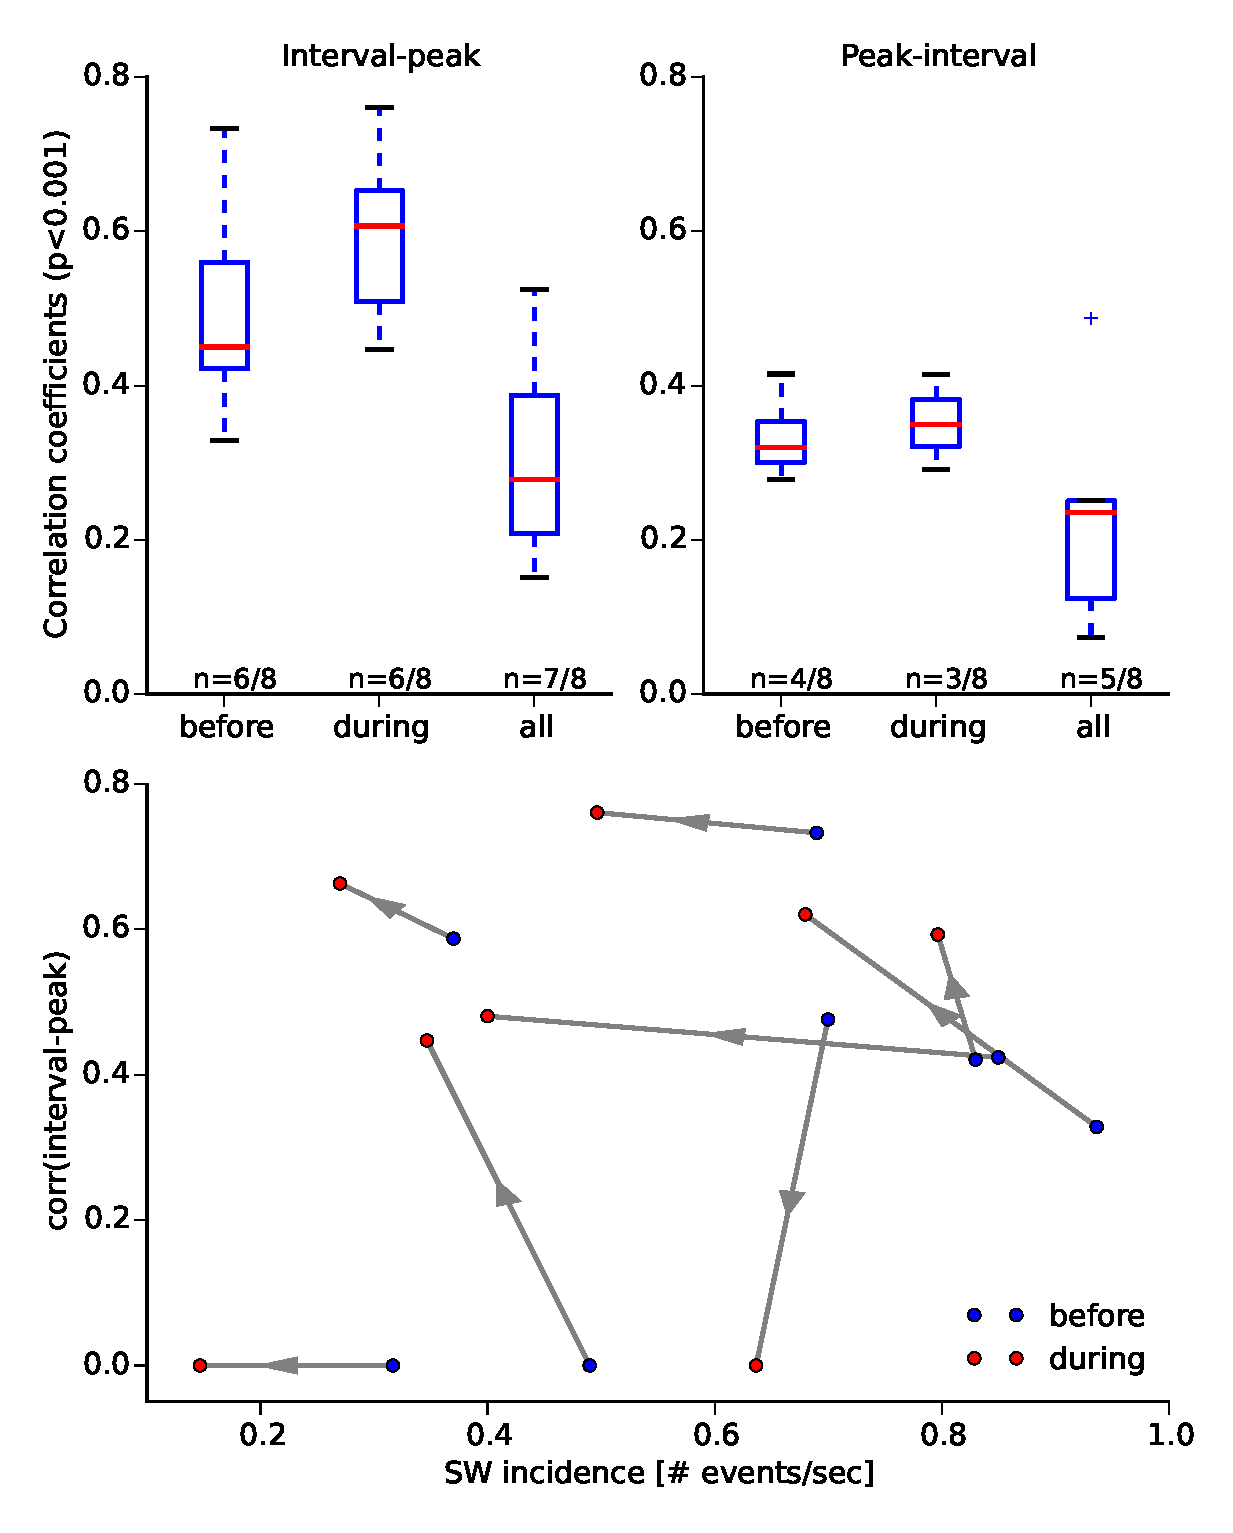
\includegraphics[width= 30pc]{gabazine_SCsumm.eps}
      \caption{
        Gabazine effect on the serial correlations. \textbf{top:} Serial
        correlation before and during gabazine are calculated in 5-minute long
        time windows, where $n$ shows the number of recordings with significant
        correlations ($p<0.001$) before gabazine application (before), during
        application (during), and aggregated data from a whole recording (all).
        \textbf{bottom:} Serial correlations coefficients between time interval
        since last event and the following SWR peak (interval-peak) are plotted
        against recorded incidence; arrows show the change after gabazine
        application. Insignificant correlations are considered to be 0.
             }
    \label{fig:gabazine_SCsumm}
    \end{figure}

    In summary, gabazine has the counterintuitive effect of decreasing the
    incidence of SWRs. Moreover, gabazine application slightly increases the SWR
    amplitude and the serial correlation between inter-sharp-wave interval and
    the peak of the following SWR. Due to the small dataset (8 recordings), I
    can not present a conclusive evidence of the drug effects. However, it is
    interesting that decreasing the inhibitory synaptic transmission increases
    the peak of SWs in the pyramidal layer (6/8 slices, 4 of which
    significant). Ideas on how gabazine affects the generation of SWRs in the
    3-population model are discussed in a greater detail in the Discussion
    (Section~\ref{sec:disc_gabazine}). In the following section, using
    numerical and analytical modelling, I study the effects of gabazine in a
    simpler 2-population model.

  \subsection{Gabazine effects on sharp-wave incidence {\textit {in silico} }}
    \label{sec:gabazine_insilico}
    To better understand how gabazine affects the incidence of SWRs {\textit
    {in silico}}, I deploy the assembly-sequence concept (described in
    Chapter~\ref{chap:asss}) as a model for the spontaneously occurring
    SWs. Here, numerical simulations of balanced networks with embedded
    assembly sequences and a linear firing-rate model are used as tools to
    describe the network dynamics under the influence of gabazine.
      
    In the numerical simulations, sequences of neural assemblies consisting of
    both excitatory and inhibitory neurons are embedded into a randomly
    connected network. Recurrent connectivity ($p_{\rm rc}=0.08$) describes the
    connection probability within an assembly while a feedforward connectivity
    ($p_{\rm ff}=0.06$) is the connectivity between the excitatory neurons of
    subsequent assemblies in the sequence (sketch of network connectivity is
    shown in Figure~\ref{fig1}). With these parameters values, noise
    fluctuations in the firing rates get amplified by the feedforward structure
    resulting in spontaneous replays (Figure~\ref{fig4}). For a more
    detailed description of the numerical model and the parameter values,
    please refer to Chapter~\ref{chap:asss}.
    
    The effects of gabazine are modeled by decreasing the conductances of the
    targeted inhibitory synapses by a fixed fraction. The network dynamics is
    stable when the conductances are decreased up to $\sim 10\%$ from their
    original value, while a larger decrease leads to an epileptiform activity.
    In Figure~\ref{fig:gabazine_sim}, ``\textit{in-silico} gabazine'' decreases
    the conductance of inhibitory synapses by $5\%$, a value which is likely to
    be smaller than the effect of $100\,\rm nM$ in the experiments
    \citep{Nimmrich2005}.

    \begin{figure}
      \center
      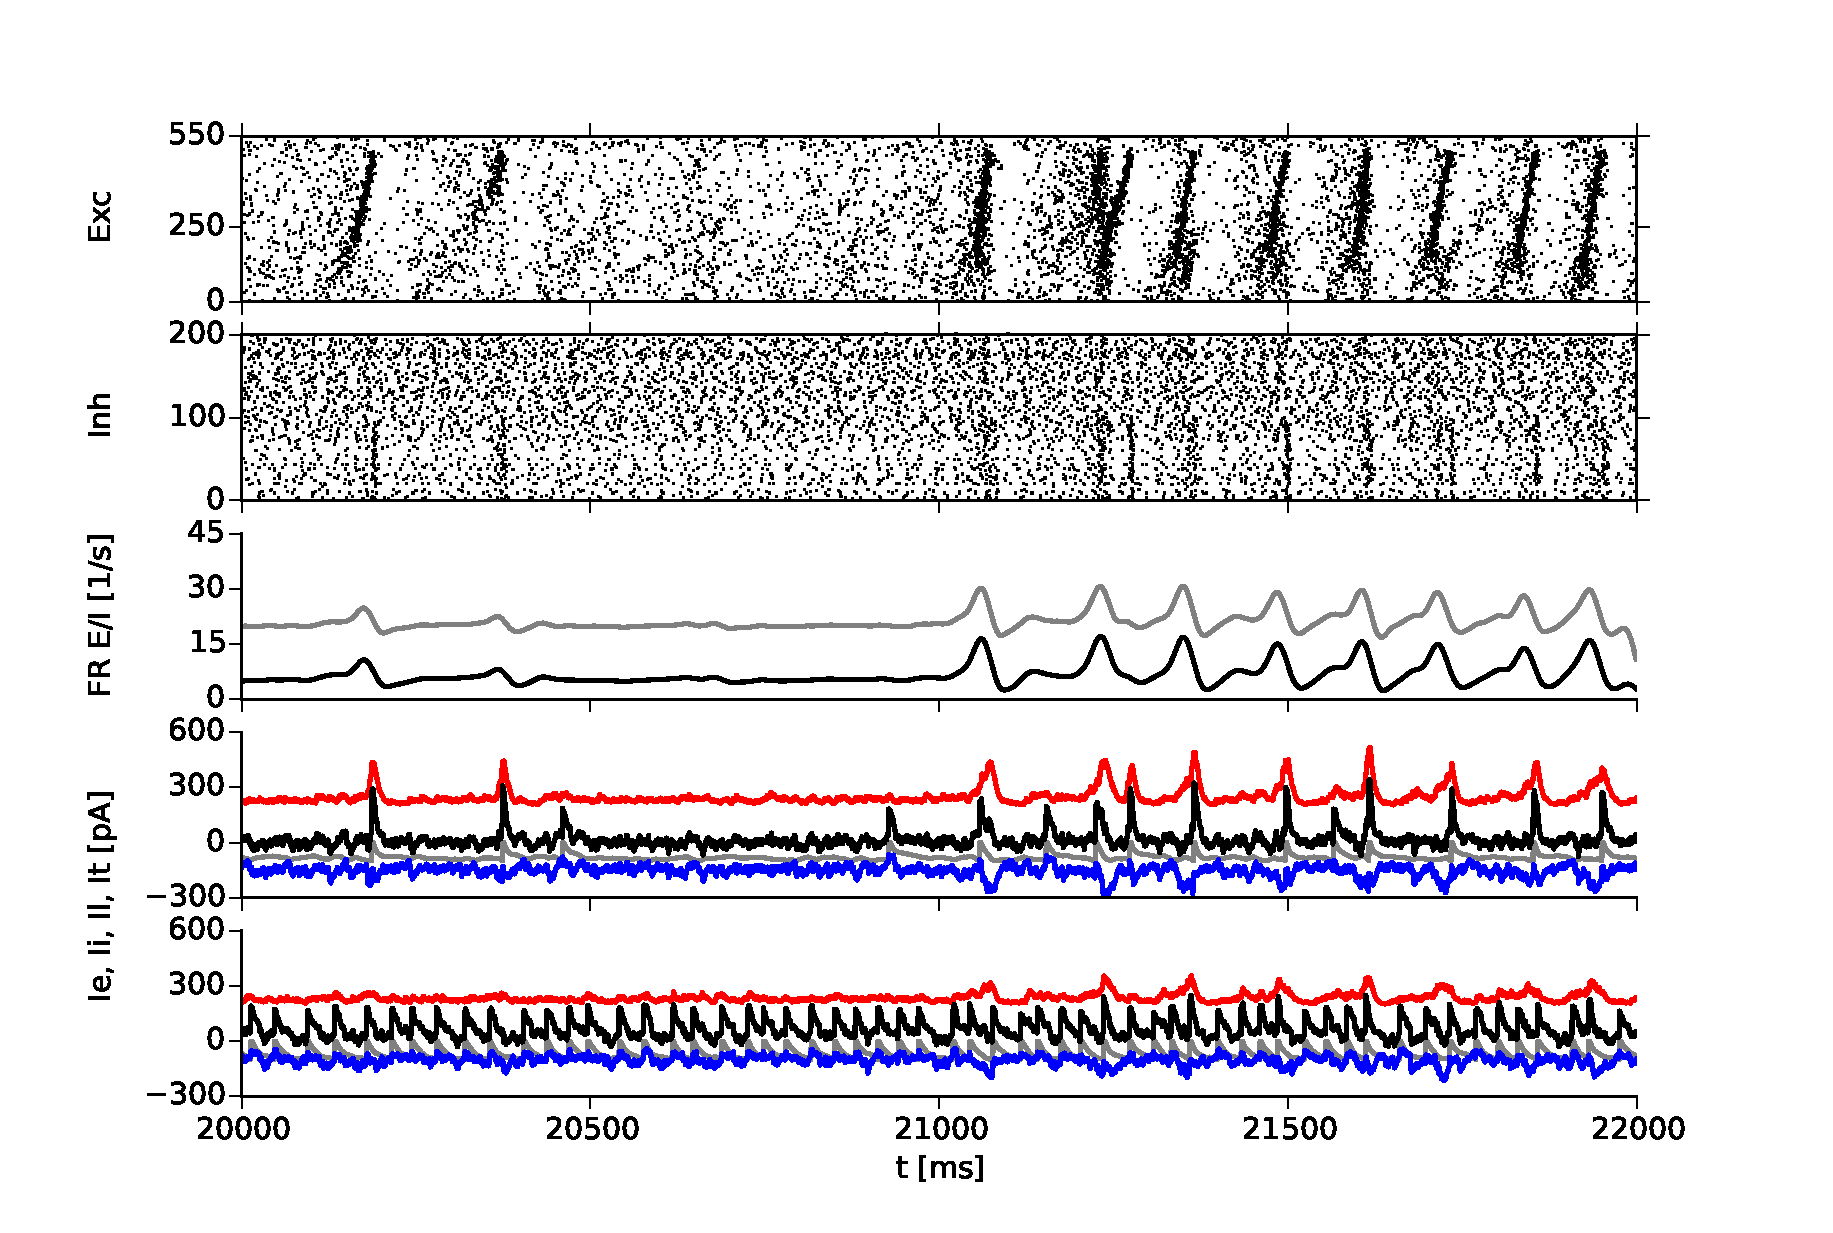
\includegraphics[width =35pc]{gabazine_sim.eps}
      \caption{
        Gabazine {\it in silico} increases the rate of spontaneous replays.
        Decreasing all inhibitory conductances (at $21^{\rm st}\, \rm second$
        by 5\%) leads to an increase in the incidence of spontaneous replays in
        balanced-network simulations. The two upper panels show raster plots of
        subpopulations of excitatory (Exc) and inhibitory (Inh) neurons, where
        each black dot denotes a spike. The middle plot shows the firing rate
        (FR) of the excitatory and inhibitory populations. The last two panels
        show the currents experienced by one excitatory and one inhibitory
        neuron. Red, blue, gray, and black colors denote excitatory (Ie),
        inhibitory (Ii), leak (Il), and total (It) currents.
            }
    \label{fig:gabazine_sim}
    \end{figure}

    Not surprisingly, \textit{in-silico} gabazine drastically increased the rate
    of spontaneous replays of assembly sequences in the modelled network. This
    is illustrated in Figure~\ref{fig:gabazine_sim}, where gabazine is applied
    to all inhibitory synapses after the $21^{\rm st}$~second of the
    simulation. The top two panels show raster plots of example excitatory and
    inhibitory neurons; black dots show individual spikes, and black
    stripes are bursts of synchronous activity during which many neurons fire in
    close temporal proximity. The replays during these activity bursts are used
    as a model of the SWR events. The frequency of these population
    events is increased immediately after the simulated gabazine infusion, as
    seen in the number of replays (the top panel), and in the firing rates
    (third panel). This result is in direct opposition with the gabazine
    effects that are reported \textit{in vitro}
    (Section~\ref{sec:gabazine_invitro}).

    Can a relatively simple two-populations balanced network explain the
    gabazine-associated decrease of SWR incidence reported in experiments?
    $\rm GABA_A Rs$ are known to be complex channels
    with five subunits that can come in various combinations (for the curious
    readers, see Section~\ref{sec:gabaa}). The expressed subunits largely
    determine the receptor properties, i.e., time constants, affinity to GABA
    and other neurotransmitters. For example tonic $\rm GABA_A R$ are
    insensitive for gabazine \citep{Bai2001, Yeung2003, Behrens2007} at low
    concentrations while phasic $\rm GABA_A Rs$ show various affinities
    depending on the subunit expression. The subunit expression is largely
    determined by the type of the postsynaptic neuron and by the location of
    the channels on the morphological tree \citep{Sieghart2002}. One hypothesis
    to explain the gabazine-associated decrease of SWR events relies on the
    assumption that gabazine has differential effects on the different $\rm
    GABA_A$ synapses. And more specifically, if inhibitory-to-inhibitory
    synapses are affected to a larger degree than the inhibitory-to-excitatory
    synapses, one would expect a network that is less disinhibited, and thus,
    the excitatory population receives more inhibition resulting in smaller
    firing rates. In what follows, I test whether such assumptions would really
    decrease the incidence of modeled events.

    As a toy example in numerical simulation, I consider the extreme case where
    gabazine affects the inhibitory-to-inhibitory synapses only.
    \textit{In-silico} gabazine indeed decreases the firing rate of the
    excitatory neurons (Figure~\ref{fig:gabazine_sim_giionly}, top panel).
    However, the network shows also a decrease in the firing rate of the
    inhibitory population as well.  How is it possible that excitatory neurons
    receiving weaker inhibition (smaller input from inhibitory population),
    fire less? To better understand the effects of gabazine, further, I present
    an analytical approach.
    
    \begin{figure}
      \center
      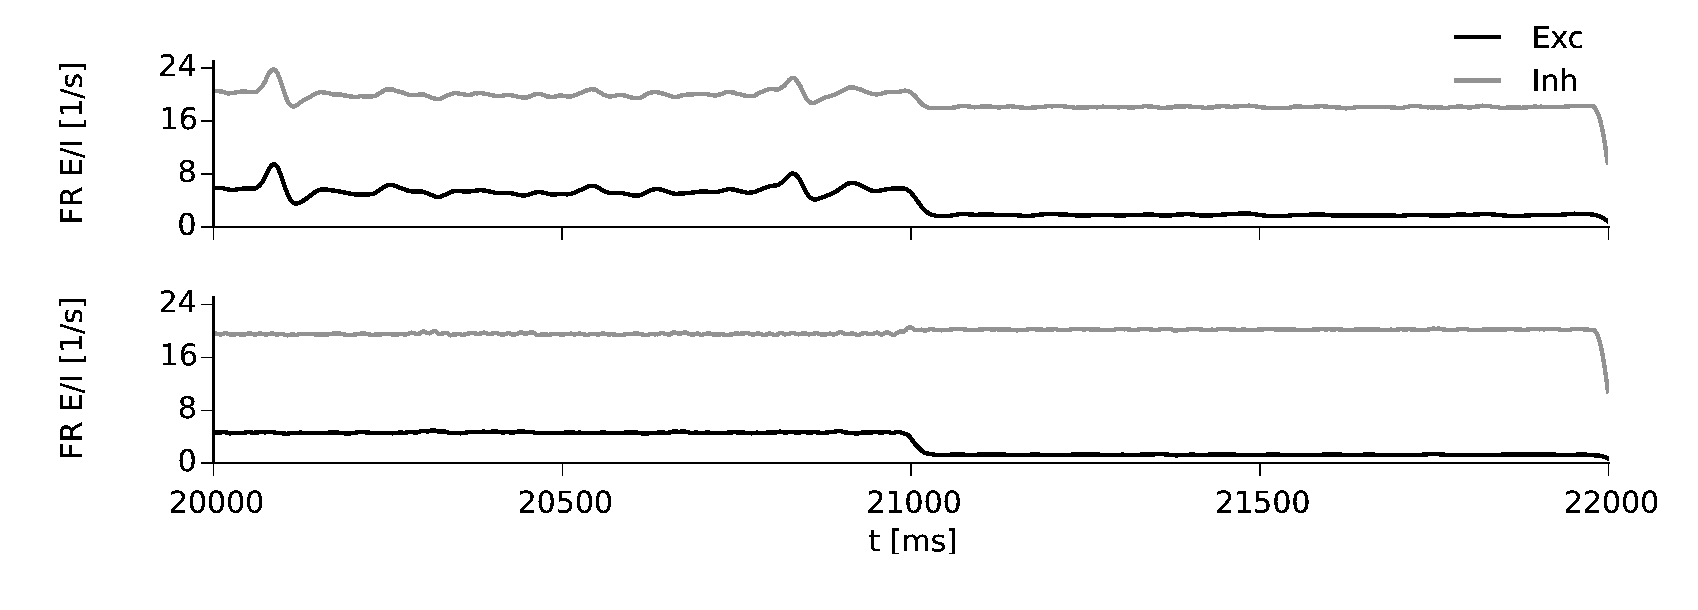
\includegraphics[width =30pc]{gabazine_sim_gii.eps}
      \caption{
        Gabazine \textit{in silico} applied only to inhibitory-to-inhibitory
        synapses decreases the rate of spontaneous replays. \textbf{top:}
        Spontaneous replays occur during the peaks of the excitatory and
        inhibitory firing rates. Decreasing the inhibitory-to-inhibitory
        conductances (at $21^{\rm st}\, \rm second$ by 5\%) decreases the
        firing rates and abolishes the spontaneous replays in balanced-network
        simulations. \textbf{bottom:} Gabazine applied only on
        inhibitory-to-inhibitory synapses can result in decrease of excitatory
        and increase of inhibitory firing rates, when excitatory-to-excitatory
        synapses are very weak in comparison to all other synapses. Here
        $g^{EE}=0$.
      }
    \label{fig:gabazine_sim_giionly}
    \end{figure}

    To capture the dynamics of the simulated network, I apply a linear model to
    a two-population balanced network and analyse how the firing rates depend
    on gabazine. The network dynamics is described by a system of differential
    equations:
    \begin{equation}
      \begin{split}
        \tau \frac{\text{d}r^E}{\text{d}t} &= - r^E + w_{\rm ee} \, r^E -w_{\rm ei} \, r^I + I_0\\
        \tau \frac{\text{d}r^I}{\text{d}t} &= - r^I + w_{\rm ie} \, r^E -w_{\rm ii} \, r^I + I_0\\
      \end{split}
      \label{eq:balanced_net}
    \end{equation}
    where the notation is as in Chapter~\ref{chap:asss}. $r^E$ and
    $r^I$ are excitatory and the inhibitory firing rates, respectively. The
    connection from populations $x$ to $y$ is described by a dimensionless
    connection weight variable $w_{\rm yx}$ ($x,y = e, i$). The population time
    constant is $\tau$, and the external input to the populations is denoted
    with $I_0$.

    Assuming that the network is in a steady state, then the rates are
    constant, i.e., $ \frac{\text{d}r^E}{\text{d}t} = 0$ and
    $\frac{\text{d}r^I}{\text{d}t} = 0 $. In this condition, one can express
    the stationary solution:
    \begin{equation}
      \begin{split}
        r^E &= \frac{(1+w_{\rm ii} - w_{\rm ei})}{w_{\rm ie}w_{\rm ei} -
                (1+w_{\rm ii})(-1+w_{\rm ee})} I_0 \\
        r^I &= \frac{(1+w_{\rm ie} - w_{\rm ee})}{w_{\rm ie}w_{\rm ei} -
                (1+w_{\rm ii})(-1+w_{\rm ee})} I_0
      \end{split}
      \label{eq:balanced_sol}
    \end{equation}
  
    To estimate how the gabazine-induced decrease of inhibitory connections
    affects the firing rates, we can look at the derivatives of the
    steady-state rates in respect to the gabazine concentration $c_{\rm gbz}$:
    \begin{equation}
      \frac{\partial r^E}{\partial c_{\rm gbz}} =
      \frac{\partial r^E}{\partial w_{\rm ei}} \cdot \frac{\partial w_{\rm ei}}{\partial c_{\rm gbz}} + 
      \frac{\partial r^E}{\partial w_{\rm ii}} \cdot \frac{\partial w_{\rm ii}}{\partial c_{\rm gbz}}
      \label{eq:re_chain}
    \end{equation}
    and
    \begin{equation}
      \frac{\partial r^I}{\partial c_{\rm gbz}} =
      \frac{\partial r^I}{\partial w_{\rm ei}} \cdot \frac{\partial w_{\rm ei}}{\partial c_{\rm gbz}} + 
      \frac{\partial r^I}{\partial w_{\rm ii}} \cdot \frac{\partial w_{\rm ii}}{\partial c_{\rm gbz}}.
      \label{eq:ri_chain}
    \end{equation}

    The partial derivatives of inhibitory weights ($w_{\rm ei}$ and $w_{\rm
    ii}$) in respect to the drug concentration $c_{\rm gbz}$ is negative due to
    the antagonist  effects of gabazine. The partial derivatives of the rates
    in respect to the inhibitory weights can easily be estimated from
    Equation~\ref{eq:balanced_sol}:
    \begin{equation}
      \begin{split}
        \frac{\partial r^E}{\partial w_{\mathrm ii}} &= 
              I_0 \frac{w_{\mathrm ei} (1 + w_{\mathrm ie} - w_{\mathrm ee})} {D^2} \\
        \frac{\partial r^I}{\partial w_{\mathrm ii}} &=
              I_0 \frac{(-1 + w_{\mathrm ee})(1 + w_{\mathrm ie} - w_{\mathrm ee})} {D^2}
      \end{split}
      \label{eq:drdwii}
    \end{equation}

    \begin{equation}
      \begin{split}
        \frac{\partial r^E}{\partial w_{\rm ei}} &=
              I_0 \frac{-(1 + w_{\rm ii}) (1 + w_{\rm ie} - w_{\rm ee})} {D^2} \\
        \frac{\partial r^I}{\partial w_{\rm ei}} &=
              I_0 \frac{-w_{\rm ie} (1 + w_{\rm ie} - w_{\rm ee})} {D^2}
      \end{split}
      \label{eq:drdwei}
    \end{equation}
    where $D=w_{\rm ie}w_{\rm ei} - (1+w_{\rm ii})(-1+w_{\rm ee})$.
    
    If we now assume that gabazine has the same effect on all inhibitory
    synapses, i.e., $\frac{\partial w_{\rm ei}}{\partial c_{\rm gbz}} =
    \frac{\partial w_{\rm ii}}{\partial c_{\rm gbz}}$, and substitute
    Equations~\ref{eq:drdwii} and \ref{eq:drdwei} in \ref{eq:re_chain} and
    \ref{eq:ri_chain}, the change of firing rate due to gabazine is:
    \begin{equation}
      \begin{split}
        \frac{\partial r^E}{\partial c_{\rm gbz}} &=
            \frac{\partial w_{\rm ii}}{\partial c_{\rm gbz}} \cdot
            I_0 \frac{-(1 + w_{\rm ii} - w_{\rm ei}) (1 + w_{\rm ie} - w_{\rm ee})} {D^2} =
            - \frac{\partial w_{\rm ii}}{\partial c_{\rm gbz}} \cdot \frac{r^E r^I}{I_0} > 0 \\
        \frac{\partial r^I}{\partial c_{\rm gbz}} &=
            \frac{\partial w_{\rm ii}}{\partial c_{\rm gbz}} \cdot
            I_0 \frac{- (1 + w_{\rm ie} - w_{\rm ee})^2} {D^2} =
            - \frac{\partial w_{\rm ii}}{\partial c_{\rm gbz}} \cdot \frac{r^I r^I}{I_0} > 0 \,\,. \\
      \end{split}
      %\label{eq:x}
    \end{equation}
    In line with the simulations, the derivatives above are always positive (if
    $\frac{\partial w_{\rm ii}}{\partial c_{\rm gbz}} < 0 $), i.e., gabazine
    always increases the rate of both excitatory and inhibitory
    populations. 

    Can this simple linear model capture the simulation results in which
    gabazine affects only inhibitory-to-inhibitory synapses? There we saw a
    decrease not only in the excitatory but also in the inhibitory firing rates
    (Figure~\ref{fig:gabazine_sim}, bottom panel). Taking the rate derivatives
    with respect to $w_{\rm ii}$ only (in Equations~\ref{eq:re_chain} and
    \ref{eq:ri_chain}, we assume that $\frac{\partial w_{\rm ei}}{\partial
    c_{\rm gbz}} = 0$), we obtain:
    \begin{equation}
      \begin{split}
        \frac{\partial r^E}{\partial c_{\rm gbz}} &=
            \frac{\partial w_{\rm ii}}{\partial c_{\rm gbz}} \cdot
            I_0 \frac{w_{\rm ei}(1 + w_{\rm ie} - w_{\rm ee})} {D^2} \\
            %\frac{\partial w_{\rm ii}}{\partial c_{\rm gbz}} \cdot \frac{w_{\rm ei}}{D} \cdot r^I \\
        \frac{\partial r^I}{\partial c_{\rm gbz}} &=
            \frac{\partial w_{\rm ii}}{\partial c_{\rm gbz}} \cdot
            I_0 \frac{(-1+w_{\rm ee}) (1 + w_{\rm ie} - w_{\rm ee})} {D^2} \,\, . \\
            %\frac{\partial w_{\rm ii}}{\partial c_{\rm gbz}} \cdot \frac{-1+w_{\rm ee}}{D} \cdot r^I \,\, . \\
      \end{split}
      %\label{eq:x}
    \end{equation}
 
    Here, the term $1+w_{\rm ie}-w_{\rm ee}$ determines the change of
    excitatory firing rate. As the connection weights are proportional to the
    conductances (e.g., $w_{\rm ee} \propto g_{\rm ee}$, see
    Chapter~\ref{chap:asss} for details), and the excitatory conductances
    used in the simulations are all equal $g_{\rm ee}=g_{\rm ie}$, one can see
    that $1+w_{\rm ie}-w_{\rm ee}>0$. In that case, it is easy to see that
    $\frac{\partial r^E}{\partial c_{\rm gbz}} < 0$, meaning that excitatory
    rate decreases when $w_{\rm ii}$ is depressed. This line of arguments is
    supported by the simulations, where gabazine applied only to the
    inhibitory-to-inhibitory connections decreases the excitatory firing rate
    (Figure~\ref{fig:gabazine_sim_giionly}). On the other hand, $r^I$ shows
    more interesting behaviour that depends on the excitatory weights. For
    intermediate values $w_{\rm ee} \in (1, 1+w_{\rm ie})$, the inhibitory rate
    decreases during gabazine application as well (as seen in
    Figure~\ref{fig:gabazine_sim_giionly}, top panel). For values of $w_{\rm
    ee}$ outside of this interval, one would expect increase of inhibitory
    firing after the drug infusion. As a proof of concept, networks with
    $g_{\rm ee}= 0\, \rm nS$ show that the inhibitory firing rate goes up after
    the simulated drug application (Figure~\ref{fig:gabazine_sim_giionly},
    bottom panel).% (c=.13, w is 2.6???)
    %To test again whether low/high wee increases ri!!!!
    %I tested that by using lower (5 times smaller than default)
    %and higher (5 times larger than default) excitatory-to-excitatory
    %connectivity in the numerical model and found that inhibitory rate is
    %indeed increased (not shown here).

    To summarize the results from this section, by using numerical simulations
    and a linear analytical description, I showed that in a balanced network a
    gabazine application is increasing the firing rates of both inhibitory and
    excitatory populations if all inhibitory synapses are similarly affected by
    the drug. This increase of firing leads to a higher incidence of
    spontaneous replays, which is in odds with the decrease of SWR incidence
    observed {\textit{in vitro}}. Therefore, I tested whether a differential
    effect of gabazine on different synapses can explain the experimental
    results. I considered the extreme case when gabazine affects only
    inhibitory-to-inhibitory synapses and showed that in this case the firing
    rate of the excitatory population can decrease. This result suggests that a
    stronger effect of gabazine on the inhibitory-to-inhibitory synapses can
    explain the decreased SWR incidence after gabazine application {\textit{in
    vitro}}.
    
    Here I examine a minimal model consisting of only two populations, which
    can nevertheless provide some means for studying \textit{in-vitro} models.
    A similar approach can also be applied to the more accurate 3-population
    nonlinear model currently developed by Roberta Evangelista, and utilized to
    examine in what conditions gabazine decreases the network excitability. Is
    it possible that in the 3-population model, a gabazine application to all
    inhibitory synapses can decrease the rate of spontaneous events? Or would
    it be required that the disinhibitory synapses (from PVBC to the mysterious
    inhibitory neurons) are affected to a larger degree?

    A strong assumption in the foundation of the current framework is that the
    decrease of SWR incidence is due to a decrease of firing of the excitatory
    population. Whether this is indeed the case can be tested in
    \textit{in-vitro} experiments. It is also not known how gabazine affects
    the firing of the inhibitory populations. Numerical and analytical results
    show that gabazine applied only on the inhibitory-to-inhibitory connections
    can decrease not only the excitatory but also the inhibitory firing rates.
    This result is interesting by its own as it demonstrates that intuitive
    interpretations of a relatively simple model can be misleading and should
    be used with caution.
    
  \subsection{Involvement of $\rm GABA_B$ receptors in sharp-wave ripples}
    SWRs are huge population events where the vast majority of interneurons are
    firing with increased rates, and single interneurons often fire multiple
    times during the event \citep{Klausberger2009, Hajos2013}. It has been
    shown that the repetitive firing of interneurons can activate extrasynaptic
    $\rm GABA_BRs$, possibly through increased concentrations of ambient GABA
    in the extracellular space \citep{Scanziani2000, Wang2010}. The inhibition
    from $\rm GABA_B Rs$ is relatively slow, lasting several hundreds of
    milliseconds, which is close to the time scale of the typical inter-SWR
    intervals. Here, I study the possibility that the relatively long time
    intervals between SWR events are determined by $\rm GABA_B Rs$.

    First, to investigate whether $\rm GABA_BRs$ are involved in the SWR
    incidence in the {\textit{in-vitro}} model, I analysed extracellular
    recordings where the $\rm GABA_B R$ antagonist SCH50,911 (further referred
    as SCH) was applied in slices. The number of analysed slices is 12 (see the
    Methods section). An example of the SCH effects in a slice is shown in
    Figure~\ref{fig:gB_example}. The drug affects the network dynamics already
    during the first minute of application by increasing the incidence of
    spontaneous SWRs (Figure~\ref{fig:gB_example}, top panel). An independent
    two-sample t-test of the incidence (measured as number of events per sweep
    in confined 5-minute time intervals) shows a significant increase of
    incidence (p-value $<10^{-7}$). Other main properties, such as peak
    amplitude and duration are decreased after SCH application (p-values
    $<10^{-10}$, and $<10^{-3}$, respectively).
    
    \begin{figure}
      \center
      %\includegraphics[width =35pc]{19march13_slice1.png}
      \includegraphics[width =35pc]{20jan12_slice2_new.png}
      \caption{ 
        Extracellular recording from the pyramidal layer of CA3 area where the
        $\rm GABA_B R$ antagonist SCH50,911 is applied to a hippocampal slice.
        The time of drug application is denoted with a horizontal red bar. The
        top panel shows the SWR incidence in time with a minute time resolution.
        The two panels below show the SWR peaks amplitude, where ``fil'' and ``raw''
        stand for band-passed filtered ($\sim 5-50\, \rm Hz$, for details see
        the Methods section) and raw voltage traces, respectively; units are in
        mV. The gray dots represent single events, and the black lines
        represent the mean and the standard deviation of the amplitude peak in
        a minute time window. Analogously, the forth panel shows the SWR
        duration in milliseconds. The panels on the bottom row show all events
        before, during, and after drug application overlaid in gray,
        and the mean wave-forms are in black. The right-most panel shows a
        comparison between the mean events from before and during SCH
        application.
              }
    \label{fig:gB_example}
    \end{figure}

    Blocking the $\rm GABA_B Rs$ resulted in increase of the average incidence
    of spontaneous SWRs from all slices ($\sim 50\%$ on average). The drug
    effects are visible already in the first minute after the application and
    saturate around 2-3 minutes later (Figure~\ref{gB_summ}, top panel). To
    better assess the effects of SCH, further, the analysis focuses on the
    events in 5-minute long time windows, i.e., in the intervals [-5, 0]
    minutes, that is before and [2, 7] minutes, that is during drug
    application. Comparing the data from these two intervals shows that SCH
    increases the incidence in every recording (10/12 show a significant
    increase; independent 2-sample t-test, $p<2 \cdot 10^{-3}$). On average,
    SCH resulted in a decrease of SWR peak amplitudes (Figure~\ref{gB_summ},
    bottom middle panel), where 6/12 slices show a significant decrease
    ($p<10^{-3}$), and in 2/12 slices the amplitudes were increased
    ($p<10^{-3}$). The SWR duration also decreased on average, but this change
    is not significant ($p>0.01$ in 11/12 slices). While the result for every
    recording varies depending on the exact 5-minute time windows that are used
    for the analysis, the summary results do not change qualitatively.
    
    \begin{figure}
      \center
      \includegraphics[width =30pc]{SCH_all.eps}
      \caption{
        The $\rm GABA_BR$ antagonist SCH50,911 affects SWRs. {\bf top}:
        SWR incidence in time aggregated from all recordings ($n=12$), where the
        incidence is normalized to 1 by dividing by the mean incidence before
        the drug application. The red bar shows the time of drug application.
        {\bf bottom:} The average SWR incidence, peak and duration measured in
        5-minute time windows before ([-5, 0] minutes) and during ([2, 7]
        minutes) SCH application for each slice are denoted with black dots.
        The red dots are the averages from all slices.
            }
    \label{gB_summ}
    \end{figure}

    Next, I inquire whether blocking $\rm GABA_B Rs$ affects also the serial
    (interval-peak) correlation between events. At first glance the pooled data
    does not reveal any change in the correlations, as the correlation
    distributions from before and during SCH application
    (Figure~\ref{gB_SCsumm}, top panels) are statistically similar. However,
    looking at the effects in the individual recordings
    (Figure~\ref{gB_SCsumm}, bottom panel) one can see that there is a decrease
    of serial correlation after drug application in 10 out of 12 slices (the 2
    remaining recordings show no significant correlations).

    \begin{figure}
      \center
      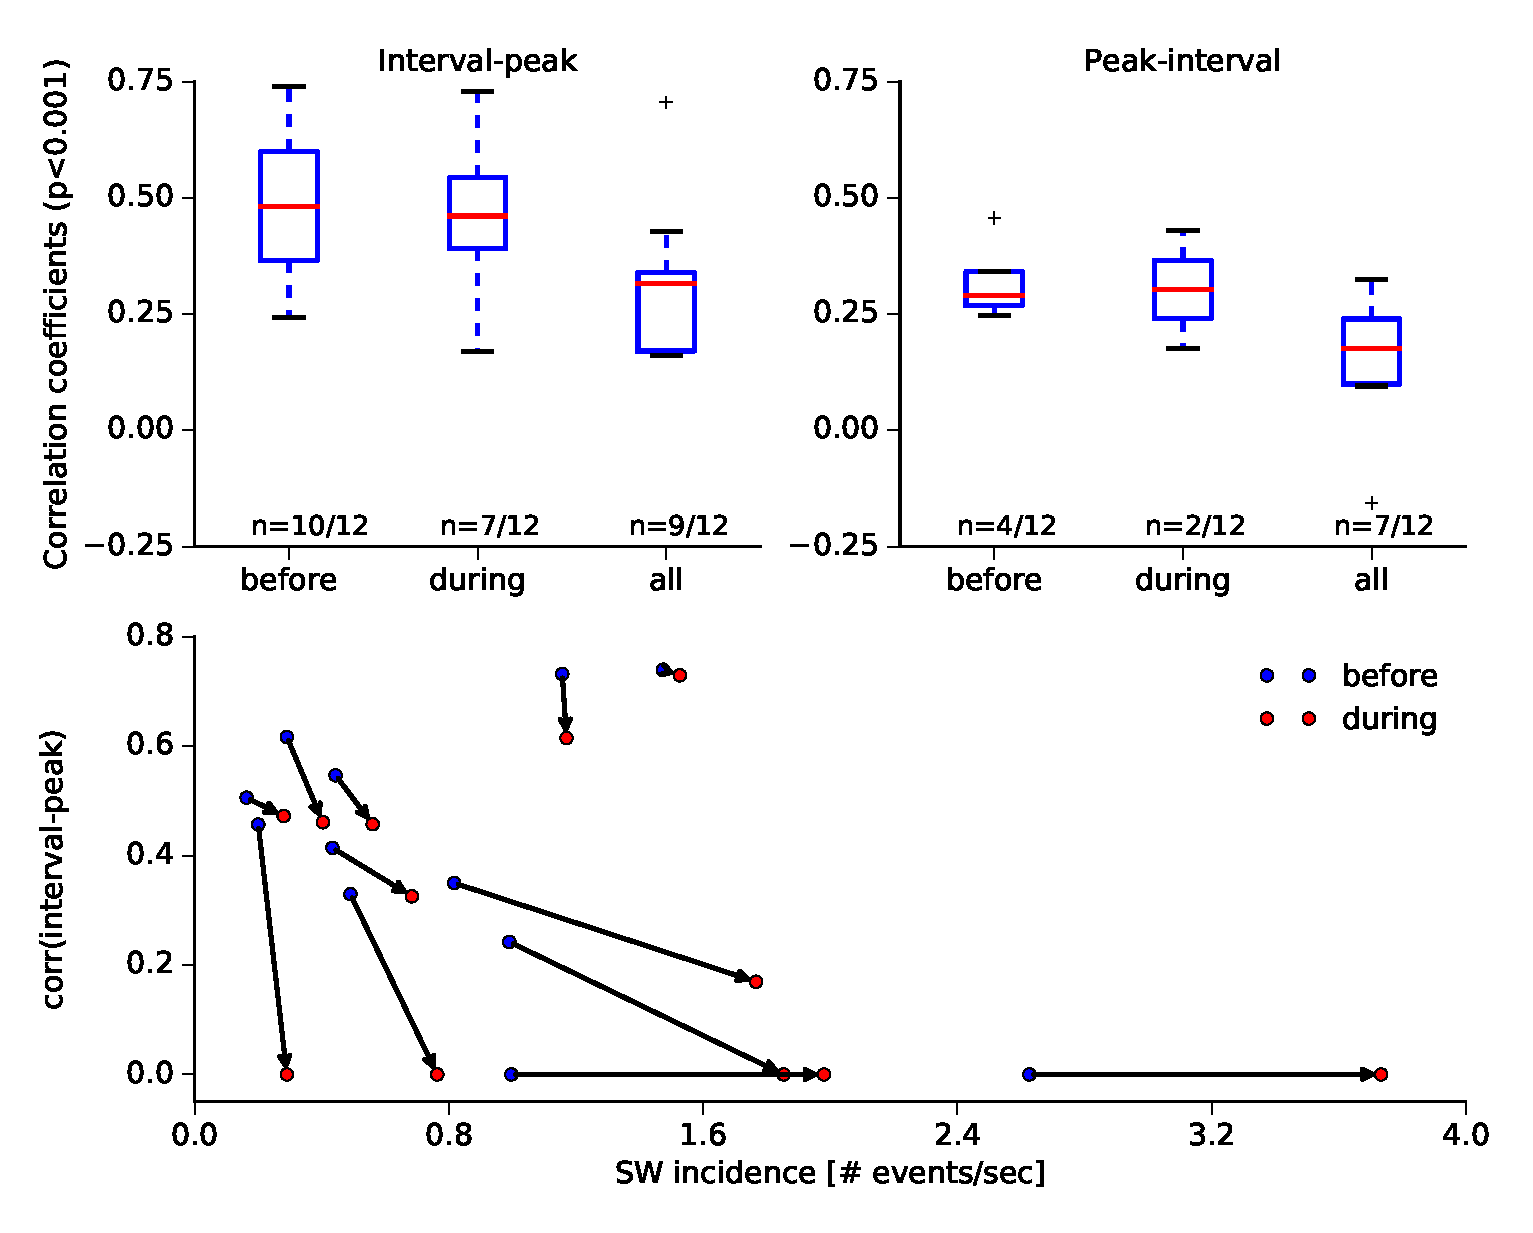
\includegraphics[width =30pc]{SCH_SCsumm.eps}
      \caption{
        $\rm GABA_BR$ antagonist SCH50,911 effect on the serial
        correlations. \textbf{top:} Serial correlation before and during
        SCH are calculated in 5-minute long time windows, where $n$ shows
        the number of recordings with significant correlations ($p<0.001$)
        before SCH application (before), during application (during), and
        aggregated data from the whole recording (all). \textbf{bottom:} Serial
        correlations coefficients between time interval since last event and
        the following SWR peak are plotted against recorded incidence; arrows
        show the change after SCH application.
            }
    \label{gB_SCsumm}
    \end{figure}

    To summarize the findings above, $\rm GABA_B Rs$ are taking part in the SWR
    modulation. In contrast to previous reports \citep[i.e.,][]{Hollnagel2014,
    Hofer2015}, the analysed data shows that $\rm GABA_BR$ antagonist
    (SCH50,911) increases the incidence of spontaneous SWR events. However, due
    to the small increase in incidence ($\sim 50\%$), the $\rm GABA_BR$ is not
    the only factor controlling the time between events as hypothesized
    initially. This result suggests that there are other mechanisms different
    than $\rm GABA_B$ that act on slow time scales and are involved in
    controlling the incidence. Moreover, application of the $\rm GABA_B Rs$
    antagonist results in a decrease of the SWR peak amplitudes and in a
    decrease in the serial correlations between interval and peaks. To
    investigate how do $\rm GABA_B Rs$ influence the SWR incidence, it is worth
    having a closer look at the possible involvement of the different $\rm
    GABA_BRs$.

  \subsection{Role of postsynaptic $\rm GABA_B$ receptors}
    It is been shown that a repetitive firing of certain interneurons can evoke
    slow and strong inhibition due to activation of postsynaptic or
    extrasynaptic $\rm GABA_BRs$ on pyramids \citep{Scanziani2000,
    Gassmann2012}. As SWRs are population events that recruit many neurons, and
    especially the perisomatic targeting interneurons \citep{Klausberger2009,
    Hajos2013}, it is likely that ambient GABA in this region is increased
    \citep{Hollnagel2014, Lang2014}. Next, I ask whether $\rm GABA_BRs$ located
    postsynaptically on pyramidal cells are indeed activated after SWs, and
    whether they play any role in the modulation of SWs. To test this
    hypothesis, here I analyse data from simultaneous (paired) extracellular
    and intracellular recordings (kindly sponsored by Nikolaus Maier) performed
    in the stratum pyramidale of the hippocampal CA3 area and a pyramidal cell
    in the CA3, respectively. By averaging the intracellular traces across
    events, we can see that pyramidal cells exhibit a rich membrane potential
    dynamics during SWR events, with various combination of depolarization and
    hyperpolarization (Figure~\ref{fig:intra_means}, top panel). A slow,
    possibly $\rm GABA_BR$-mediated hyperpolarization is present in a few
    recordings, but is not is not visible in the average trace from all cells
    (Figure~\ref{fig:intra_means}, top panel, thick black line). In the
    recordings that show a slow hyperpolarization (4 out of 13 cells,
    Figure~\ref{fig:intra_means}, bottom panel) the trough in the membrane
    potential is around $200 \, \rm ms$ after the population event and lasts
    for about $500 \, \rm ms$. Interestingly, one recording reveals
    well-pronounced slow as well as fast inhibition (red trace).

   \begin{figure}
      \center
      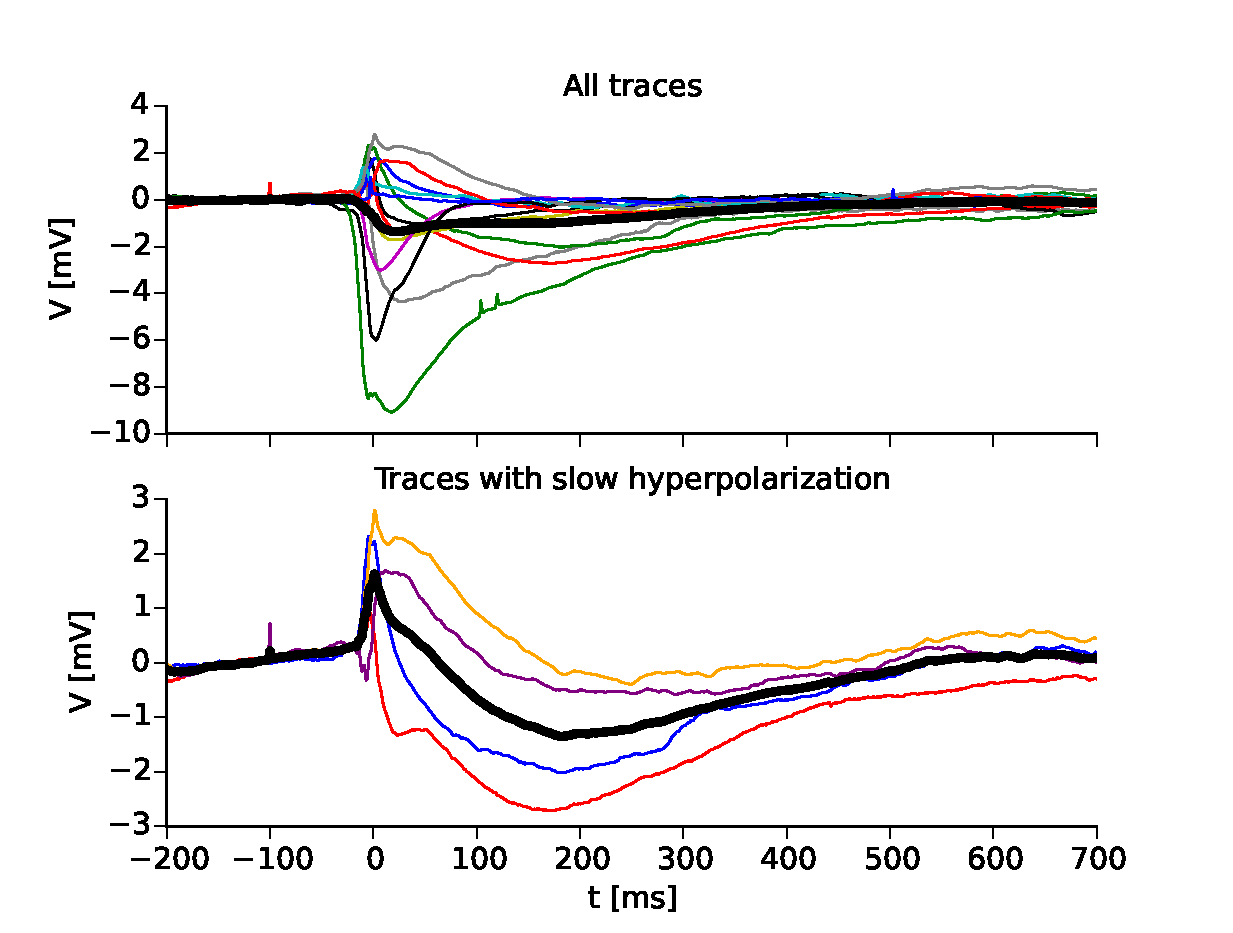
\includegraphics[width =25pc]{mean_intras.eps}
      \caption{ 
        Patch-clamp recordings from pyramidal cells during SWRs. {\bf top:}
        Mean voltage traces associated to SWRs from each slice are color coded;
        the thick black line is the mean of the means. {\bf bottom:} Mean
        voltage traces of cells that show slow, possibly $\rm GABA_BR$-mediated
        hyperpolarization (4/13 cells). Membrane potentials are normalized by
        subtracting the mean depolarization in a 200-millisecond interval
        preceding the event.
              }
      \label{fig:intra_means}
    \end{figure}

    Is the slow hyperpolarization correlated in any way with the amplitude of
    the SWs? To test this, I separated the events in each recording in two
    groups: big and small events, i.e., the 30\% largest SWR peaks and 30\%
    smallest events, respectively. Plotting the mean intracellular trace during
    small and big events, shows that the SWs with larger amplitudes are
    associated with larger hyperpolarization (Figure~\ref{fig:intra_big_small},
    top panel). Interestingly, the mean traces before big and small events are
    virtually indistinguishable (Figure~\ref{fig:intra_big_small}, bottom
    panel), suggesting that the amount of hyperpolarization does not determine the size
    of the following event. This result holds for all four recordings that
    exhibit slow inhibition in the membrane potential.
    
    \begin{figure}
      \center
      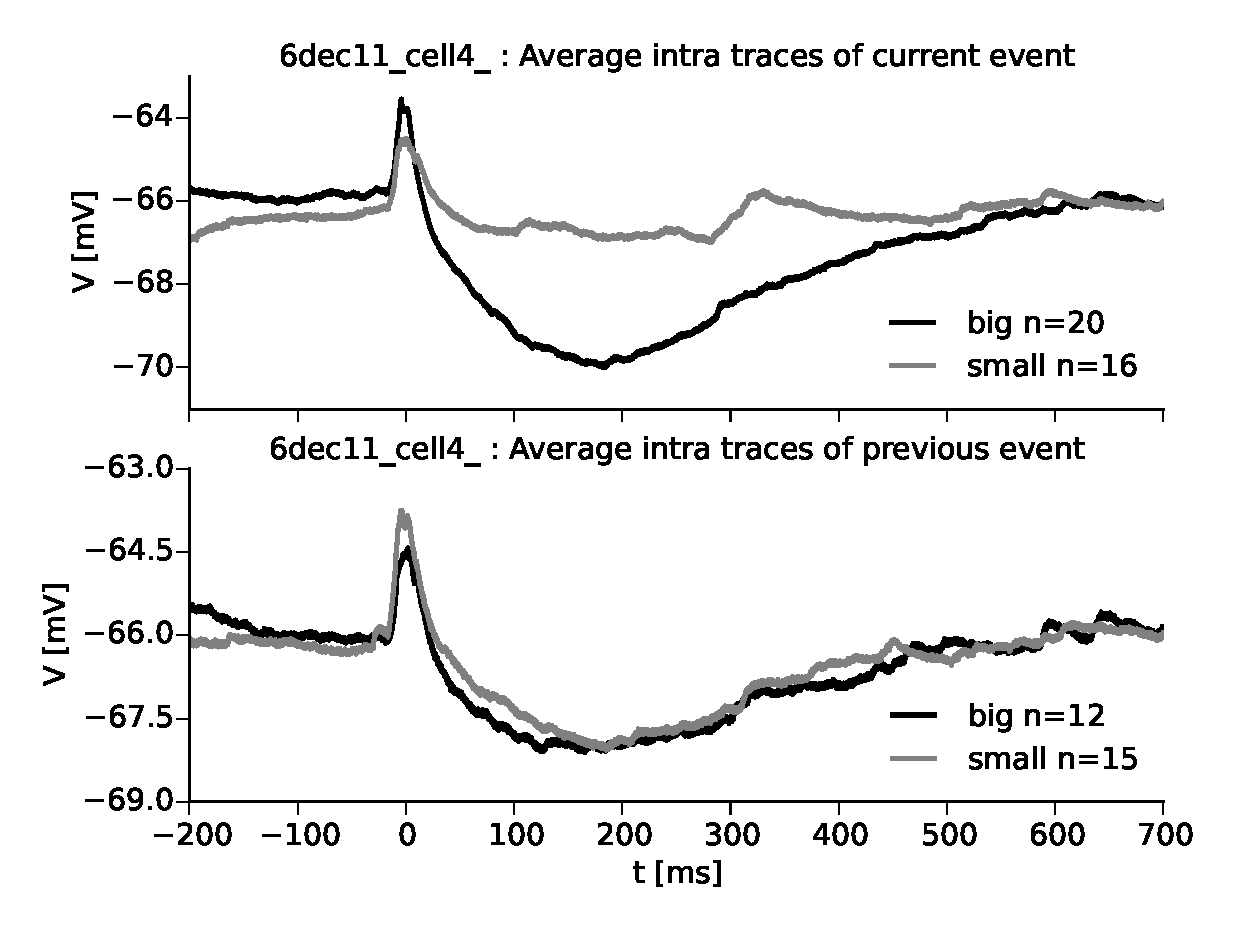
\includegraphics[width =25pc]{6dec11_cell4_000.eps}
      \caption{ 
        Sharp-waves ripples with larger peak amplitudes evoke stronger
        hyperpolarization. {\bf top:} Big events (30 \% of the largest SWR
        events) are associated with a well-pronounced slow hyperpolarization.
        Smaller events (30\% of the smallest SWRs) did not evoke a $\rm
        GABA_B$-associated response. The difference of membrane potentials
        prior to events is a recording artifact (see the Methods section). {\bf
        bottom:} There is no correlation between the depolarisation of a cell
        and the peak amplitude of the following SWR event.
              }
      \label{fig:intra_big_small}
    \end{figure}

    Moreover, the slow hyperpolarization does not affect the time interval
    until the following event (not shown here). There is a correlation between
    the inter-SWR interval and the amplitude of the following hyperpolarization,
    which is expected given the fact that longer intervals are followed by
    larger SWs, and thus, larger hyperpolarization.

    The last recording data of intracellular and extracellular recordings
    reveals that slow, possibly $\rm GABA_B$-mediated hyperpolarization occurs
    in a fraction of the CA3 pyramidal neurons \textit{in vitro}. The magnitude
    of the received inhibition is not correlated with the size or the time
    interval until the next event. Therefore, intracellular recordings suggest
    that the time interval between events is not controlled by the postsynaptic
    $\rm GABA_B Rs$ on pyramids.
 
    %decreased peak means decreased currents; however, blocking presynaptic gBR would lead to increased single IPSC/P; therefore likely that SCH decreases FR of perisomatic targeting INs during SWR events

\section{Discussion}
  In this chapter I analysed the serial correlations between sharp-wave ripple
  events measured in the stratum pyramidale of CA3 area in hippocampal slices.
  To briefly summarize, the results reveal a strong correlation between time
  interval since the last event and the peak amplitude of the following SWR
  (significant correlation in 18/20 slices, mean correlation $\sim 0.4$). On
  the other hand, there is a lower serial correlation between the events size
  and the time interval (significant positive correlation in 7/20 slices,
  significant negative correlation in 2/20 slices, mean correlation $\sim 0.2$)
  until the following event. There is not locality of the SWR events because
  multi-electrode array recordings revealed that SWR peak amplitudes are a
  non-local phenomenon, and a large SWR measured at one location is likely to
  be large in the whole CA3 region. 
  
  Application of the $\rm GABA_AR$ antagonist gabazine decreased the incidence
  of SWRs \citep[in agreement with][]{Nimmrich2005}, Moreover, gabazine
  increased the size of SWR events measured in stratum pyramidale (significant
  change in 4/8 slices), and increased the interval-peak serial correlations. 

  In contrast to previous reports \citep[i.e.,][]{Hollnagel2014, Hofer2015},
  here I showed that the $\rm GABA_BR$ antagonist SCH50,911 increased the
  incidence of spontaneous SWR events (10/12 slices). On average, the SCH50,911
  application resulted in a decrease of SWR amplitudes (significant decrease in
  6/12; significant increase in 2/12 slices) and in a decreased interval-peak
  correlation. Moreover, intracellular recordings suggested that the time
  interval between events is not controlled by postsynaptic $\rm GABA_B Rs$ on
  pyramids due to the absence of a correlation between the slow
  hyperpolarization and the inter-event interval.

  The results above do not reveal the mechanisms controlling the generation of
  SWRs, but provide some insights about the possible circuitry, which are
  discussed in detail in what follows.
    
  \subsection{Hypotheses on how gabazine affects sharp-wave ripples} 
  \label{sec:disc_gabazine}
    It has been shown that gabazine, which is a $\rm GABA_AR$ antagonist, leads
    to a lower incidence of SWRs. Here, I give an interpretation of the
    counterintuitive result that a reduction of inhibition leads to a reduction
    of SWR incidence.

    \subsubsection{Hypothesis on how gabazine affects sharp-wave amplitude} 
      An interesting observation is that the application of gabazine tends to
      increase the amplitudes of the field potential measured in stratum
      pyramidale during SWRs. Similarly, \cite{Steidl2006} reported increase of
      the stimulus-evoked field potential in the pyramidal layer after the
      application of $500\,\rm nM$ gabazine, while no significant changes were
      observed in other layers. The field potential in the pyramidal layer is
      dominated by inhibitory synaptic currents \citep{Schonberger2014}, most
      likely from the fast local perisomatic synapses \citep{Ylinen1995}.
      Therefore, I conclude that although gabazine decreases the unitary (i.e.,
      single spike activated) postsynaptic currents, there is an increase in
      the firing rate of perisomatic-targeting interneurons, resulting in a net
      increase of inhibitory currents during a SWR. The exact identity of these
      neurons is to be found. Because the parvalbumin-positive basket cells
      (PVBCs) are among the most active interneurons during SWRs, and their
      projections to the pyramidal cells (PCs) are located in the pyramidal
      cell layer (where the recordings are performed), further, I assume that
      PVBC are among the cells with increased firing rate.

    \subsubsection{Hypothesis on how gabazine affects sharp-wave incidence} 
      In the numerical simulations of the 2-population network model, the
      spontaneous replay of assembly sequences was used as a model for SWRs. As
      intuitively expected, decreasing all inhibitory conductances in the
      balanced network led to an increase of replay incidence. However, a
      differentiated role of gabazine on the inhibitory-to-excitatory (I-to-E)
      and I-to-I synapses in the simulations could replicate the original
      gabazine experiment. More specifically, if I-to-I synapses are affected
      to a larger degree than the I-to-E synapses, then the incidence of
      spontaneous bursts is decreased. Currently, it is not clear whether the
      same argument can be applied to the 3-population hypothesis (see
      Section~\ref{sec:3pop}). It may be possible that a ``gabazine application''
      to all inhibitory synapses can decrease the rate of spontaneous events in
      the non-linear 3-population model. A detailed mathematical analysis,
      similar to the one presented in Section~\ref{sec:gabazine_insilico} could
      answer these questions.

      The hypothesised increased firing of the perisomatic-targeting
      interneurons, as discussed above, can decrease the SWR incidence through
      two major pathways. First, repetitive firing of an interneuron can lead
      to excess of GABA at the synaptic cleft, leading to a diffusion into the
      extracellular space \citep{Farrant2005}. The ambient GABA can then (i)
      activate the tonic $\rm GABA_ARs$ that are especially sensitive to GABA
      \citep{Semyanov2004}, or (ii) activate $\rm GABA_BRs$ at the pyramidal
      cell bodies \citep{Scanziani2000}. Both of these extrasynaptic receptor
      types are slow in comparison to phasic inhibition and can keep cells
      hyperpolarized for longer time intervals, which are in the order of the
      inter-event time intervals. 
      
      The two pathways can explain why gabazine and thiopental, which have
      opposite effects on the inhibitory transmission, result in a similar SWR
      modulation. Both drugs lead to diffusion of GABA to the extrasynaptic
      GABAergic receptors. For example, larger concentrations of gabazine
      ($5\,\rm \mu M$) applied to hippocampal slices lead to a persistent
      hyperpolarization of the pyramidal cells of $\sim 9\, \rm mV$ below the
      membrane potential measured in control conditions \citep{Behrens2007}. It
      is not known whether this is the case with the lower gabazine
      concentrations in the SWR model analysed here, but this effect can be
      tested experimentally. Intracellular recordings can reveal whether small
      concentrations of gabazine ($\sim 100 \, \rm nM$) also lead to a
      persistent hyperpolarization. If this is the case, an additional local
      application of a tonic $\rm GABA_AR$ antagonist \citep[e.g.,
      DPP-4-PIO;][]{Boddum2014} or a $\rm GABA_BR$ antagonist could reveal the
      identity of the involved extrasynaptic receptors. In a ``reversal
      experiment'', if a GIRK-channel blocker applied after the gabazine
      reverses the SWR incidence to a control level, it would be a hint that
      gabazine modulates SWRs through activation of postsynaptic $\rm
      GABA_BRs$. Or in an ``occlusion experiment'' for example, if gabazine does
      not affect the incidence in slices with already bocked tonic $\rm
      GABA_AR$, it would suggest that the tonic $\rm GABA_AR$ are involved.

      The other major mechanism explaining SWR incidence modulation is in line
      with the numerical and analytical analysis (see
      Section~\ref{sec:gabazine_insilico}) of gabazine affecting the
      disinhibitory pathway to a larger degree compared to the inhibitory
      pathway on PCs. On the one hand, due to its antagonist properties,
      gabazine decreases the efficacies of the PVBC-mIN synapses. On the other
      hand, the increased spiking of PVBC during events would lead to a
      stronger short-term depression on the PVBC-mIN synapses compared to
      control conditions. Both mechanisms could contribute to the elevation of
      the mINs firing rate, and thus, to the increase of dendritic inhibition
      on pyramidal neurons after drug application. The plausibility of gabazine
      affecting the disinhibitory pathway can be tested experimentally, once
      the mIN population is identified.

    \subsubsection{Hypothesis on how gabazine affects the serial correlations}
    What is the mechanism of the observed gabazine-mediated increase of the
    interval-peak correlations in the majority of slices? This observation is
    puzzling: for a decreased incidence, one would expect decreased
    correlations because of the longer time for synaptic recovery from STD.
    However, the hypothesised higher firing rate of PVBCs (after gabazine)
    leads to a stronger synaptic depression, and thus, to a longer recovery
    time of the PVBC afferent synapses (PVBC-PC, particularly). This implies
    that in `control' \textit{in-vitro} experiments, the STD after SWR events
    is not saturated to its maximal value.
      %to a larger
      %degree than the increase on the inter-SWR time interval.
      
      %--- make up a figure sketch of the idea: STP, PVBC FR --- here or in the discussion
      %Local gabazine puff decreases the SWR peaks in Schilinglof, but is also
      %decreases the MU firing \ref{fig:schlingloff_gabazine}. Cells are more
      %inhibited? However in another experiment the same authors measured PVBCs in
      %a loose patch and show that their FR is increased. This suggests some

    \subsubsection{Other mechanisms} 
      % glycine
      Up to this point, it has been considered that gabazine targets
      exclusively the $\rm GABA_ARs$. However, it has been shown that gabazine
      (as well as bicuculline) blocks also the glycine receptors
      \citep{Wang2005, Li2007}. Glycine receptors are ionotropic inhibitory
      receptors that (upon activation) produce chloride flow into the cell
      membrane. They are present in the hippocampus in smaller quantities
      relative to other brain areas \citep{denPol1988} and cluster around the
      inhibitory synapses on pyramidal cells and interneurons \citep{Levi2004}.
      Whether the incidence of SWRs is influenced by gabazine blocking the
      glycine receptors can be tested in experiments. In particular, does the
      application of a glycine receptor antagonist occludes the effect of
      gabazine or bicuculline?
      %glycine receptors \citep{Shirasaki1991} 
      %and SK-type potassium channels \citep{Pedarzani2001}.  gabazine influencing glycine
      %Debarbieux98: BIC blocks SK ca chans

  \subsection{Hypothesis on how $\rm GABA_B$ receptors influence the sharp-wave incidence} 
    Currently, it is not known through what mechanisms the $\rm GABA_BRs$
    influence the SWR incidence. In contrast to previous reports
    \citep[e.g.,][]{Hollnagel2014, Hofer2015}, the slice recordings analysed
    here showed a significant increase of SWR incidence after application of the
    $\rm GABA_BR$ antagonist SCH50,911. On the other hand, agonists of $\rm
    GABA_BR$ led to a decrease of SWR incidence \citep{Maier2012,
    Hollnagel2014}. Five different $\rm GABA_BR$-mediated pathways can explain
    these results in the framework of the phenomenological 3-population model.
     
    \begin{itemize}
      \item \textbf{Postsynaptic $\rm GABA_BRs$ on PCs.}
        A possible location of $\rm GABA_BR$ is on the postsynaptic sites on
        pyramidal cells. It is been shown that the activation of these
        receptors leads to slow IPSPs with high amplitudes in CA3 principal
        cells \citep{Knowles1984}. Such hyperpolarization would result in a
        lower spontaneous firing rate of the PC population, and thus, a lower
        incidence of SWs. There are experimental evidences that $\rm GABA_BR$
        are located along the whole somato-dendritic axis on the principal
        cells, with highest concentrations in the stratum radiatum and
        lacunosum moleculare layer \citep{Degro2015}. Moreover, $\rm GABA_{B1}$
        receptors cluster with GIRK channels at the dendritic spines of PCs
        mostly in the stratum oriens, stratum radiatum and lacunosum moleculare
        \citep{Kulik2006}. The activation of postsynaptic $\rm GABA_BRs$
        requires a repetitive firing of one or more presynaptic interneurons
        \citep{Scanziani2000}.

      \item \textbf{Postsynaptic $\rm GABA_BRs$ on PVBCs.}
        Because of the hypothesised disinhibitory role of the PVBCs, 
        postsynaptic $\rm GABA_BRs$ on the PVBCs would also suppress the
        initiation of SWs upon activation and facilitate SWR generation upon
        suppression. Immunolabeling shows that $\rm GABA_BRs$ are co-localised
        with GIRK channels predominantly at the dendrites and the soma of the
        $\rm PV^+$ interneurons \citep{Booker2013}, and to a smaller degree on
        the axons. Moreover, slow $\rm GABA_B$-mediated IPSPs are present in
        the perisomatic-targeting, but not in the dendritic-targeting $\rm
        PV^+INs$ \citep{Booker2013}.

      \item \textbf{$\rm GABA_B$ heteroreceptors on PCs.}
        Activation of $\rm GABA_BRs$ at the presynaptic side of the recurrent
        excitatory synapses suppresses glutamate release, and thus, the network
        excitability. It has been shown that both $\rm GABA_{B1}$ and $\rm
        GABA_{B2}$ are expressed at the presynaptic terminals of CA3 recurrent
        synapses \citep{Lopez2004}, and that these receptors can modulate the
        AMPA receptors \citep{Lei2003}. Moreover, GIRK channels cluster with
        $\rm GABA_{B1}$ at the excitatory axons \citep{Kulik2006}. However, the
        functionality of these receptors is not clear. For example,
        \cite{Lei2003} have shown that the baclofen-mediated inhibition of
        EPSPs is larger compared to the inhibition of IPSPs, and that the $\rm
        GABA_{B}R$ antagonist CGP55,845 enhanced the IPSPs but not the EPSPs.
        %Blocking the heteroreceptors on PCs \citep{Maier2012} ?

      \item \textbf{$\rm GABA_B$ heteroreceptors on PVBCs.}
        Activation of presynaptic $\rm GABA_BRs$ on the PC-PVBC connections
        would suppress the excitability of PVBCs, which would lead to a
        suppression of SWRs. It is been shown that presynaptic $\rm GABA_BRs$
        on the glutamatergic synapses can inhibit the excitatory transmission
        on CA3 interneurons \citep{Lei2003}, but the identity of these
        interneurons is unknown.

      \item \textbf{$\rm GABA_B$ autoreceptors on PVBC-mIN synapses.}
        Activation of $\rm GABA_BRs$ located presynaptically on the PVBC-mIN
        connections would decrease the inhibition on mINs, and thus, decrease
        the incidence of SWRs. \cite{Lei2003} have shown that inhibitory
        transmission to hippocampal interneurons is modulated by presynaptic
        $\rm GABA_BRs$. Particularly, \cite{Booker2013} showed that the output
        of perisomatic-targeting $\rm PV^+$ interneurons is modulated by $\rm
        GABA_BRs$.
    \end{itemize}

    There are anatomical evidences supporting each of the hypotheses described
    above. However, which, if any of these $\rm GABA_BRs$ are activated indeed
    during SWRs is unknown. Some experimental evidences from the literature
    point to a presynaptic modulation. For example, \cite{Hollnagel2014}
    suggest that the $\rm GABA_BR$ agonist baclofen decreases SWR incidence due
    to presynaptic glutamatergic suppression. However, the used
    \textit{in-vitro} model is different as SWs occur spontaneously just after
    a train of external stimulations, and $\rm GABA_BR$ antagonist did not lead
    to an increase in the SWR incidence. A study by \cite{Maier2012} shows that
    adenosine (activates GIRK channels, and suppresses glutamate transmitter
    release) suppresses SWRs because of presynaptic modulation.  Moreover, there
    is no evidence that the postsynaptic $\rm GABA_BR$-mediated
    hyperpolarization (on PCs) is associated with the interval until next
    spontaneous event in the intracellular recordings analysed here. However,
    data (from personal communication with Nikolaus Maier) points out that
    application of GIRK-channel blocker (SCH23,390) increases SWR incidence, and
    moreover, a later application of $\rm GABA_BR$ antagonist does not suppress
    the SWR incidence. This result suggests that the postsynaptic GIRK-coupled
    $\rm GABA_BR$ are involved in the modulation of SWs, but not the
    presynaptic ones. Moreover, the $\rm GABA_BR$ antagonist CGP52432, that
    acts predominantly on the autoreceptors \citep{Lanza1993}, did not
    influence SWR incidence in the \textit{in-vitro} model used by
    \cite{Hofer2015}. Such result hints that the reported here increase of SWR
    incidence might be not due to presynaptic $\rm GABA_BRs$ on inhibitory
    synapses.
    %In conclusion, a largely unexplored pathway of SWR modulation is $\rm GABA_B$? do this sent or remove
    
    There are more possible location sites for the $\rm GABA_BRs$ that haven't
    been discussed here. Through the prism of the 3-population model, the sites
    not mentioned here (e.g., presynaptic $\rm GABA_BRs$ on the outgoing mIN
    synapses) would modulate SWR incidence in the opposite direction as observed
    experimentally. Only the five pathways described above would lead to the
    experimentally observed effects of $\rm GABA_BR$ modulators. The question
    whether one or more of these mechanisms are deployed simultaneously is to
    be answered. Cocktails of drugs could help us to better disentangle the
    different mechanism of receptors modulation. For example, more experiments
    with a sequential application of GIRK-channel blocker and $\rm GABA_BR$ antagonist could be
    performed, where first one of the drugs applied, and after a few tens of
    minutes the other. Another experiment to test the postsynaptic modulation
    is to apply a $\rm GABA_BR$ agonist, which will decrease the incidence, and
    to apply a GIRK-channel blocker afterwards to check whether the incidence
    is normalized. If the experiments favor a presynaptic modulation, the
    differential distribution of $\rm GABA_B$ subunits (i.e., $\rm
    GABA_{B(1a,2)}$ and $\rm GABA_{B(1b,2}$) on different neurons could help
    narrow down the list of suspected receptors. However, one should be careful
    with the interpretation of the results as the effects of $\rm GABA_BR$ are
    nonlinear \citep{Brenowitz1998}. Upon activation, presynaptic
    \citep{Schwenk2010}, as well as postsynaptic \citep{Wetherington2002} $\rm
    GABA_BR$ can get desensitized.

    Another possible influence of the $\rm GABA_{B}Rs$ is through the
    modulation of short-term inhibitory plasticity, which is hypothesised to
    control the SWR incidence and amplitude. Short-term depression (STD) is
    usually mediated presynaptically \citep{Kraushaar2000}. Moreover, the STD
    of inhibitory neurons can be modulated by $\rm GABA_BRs$ \citep{Lei2003}.
    It would be interesting to find out whether STD of PVBCs is also modulated
    by the $\rm GABA_BRs$.

    In summary, activation or inactivation of $\rm GABA_BRs$ can facilitate or
    depress the spontaneous generation of SWRs, respectively. Here, I proposed
    a few possible pathways of modulation. However, unlike hypothesised
    initially at the beginning of this project, the $\rm GABA_BR$ does not seem
    to be the crucial mechanism defining the relatively long time scale between
    events.
        
  \subsection{Overview}
    After over two decades of research, the mechanisms of sharp-wave ripple
    generation are still under debate. While some of the early theories focused
    exclusively on the role of excitation (e.g., \citealp{Draguhn1998} and
    \citealp{Memmesheimer2010}, but also \citealp{Ylinen1995}), a number of
    evidences from the last years point out the importance of inhibitory
    transmission not only for the ripple oscillation, but also for the
    generation of the whole population event \citep{Maier2011, Schlingloff2014,
    Stark2014, Kohus2016}. While the build-up of excitation is an important
    requirement for the generation of spontaneous events \citep{delaPrida2006,
    Ellender2010, Schlingloff2014, Hulse2016}, SWR-like events can also be
    evoked by a spontaneous experimentator \citep{Maier2003, Nimmrich2005,
    Both2008, Kohus2016} even in the absence of excitatory transmission
    \citep{Schlingloff2014}.
    
    A phenomenological 3-population model relying on disinhibition explains
    some intriguing results from the literature. In particular, the model
    relies on a network circuit that can switch between two states: one state
    is characterised by a low firing rate of principal neurons and an unknown
    interneuron population, and another (transient) state by high firing rates
    of the principal and parvalbumin-positive basket neurons. However,
    currently the model is too general to explain all experimental findings. A
    number of possible experiments have been proposed in the preceding sections
    that can help us refine the model, and possibly validate or invalidate it. 

    To find the missing link between the SWR events and the slow time scale of
    the inter-event interval, one possibility is to look beyond the neural
    circuit. The astrocyte network, in particular, operates on a slower time
    scale \cite[$\sim 500 \,\rm ms$,][]{Sasaki2014}, and has been known to
    modulate neural activity through complex and not well-understood
    mechanisms. For example, astrocytes control neural excitability through
    gliotransmitters (e.g., glutamate, \citealp{Parpura1994}; ATP,
    \citealp{Newman2001}; GABA, \citealp{Liu2000}) and through modulation of
    the extracellular concentration of $\rm K^+$ \citep{Wang2012}. The
    astrocyte network can propagate $\rm Ca^{2+}$ waves triggered by
    neurotransmitters such as glutamate \citep[e.g.,][]{Cornell1990}.
    Recently, \cite{Zhang2017} showed that acute induction of astrocyte $\rm
    Ca^{2+}$ influx led to a suppression of neural activity on one-second time
    scale in a drosophila model. It is unclear whether similar mechanism are
    active in the hippocampus. Currently, the connections between SWRs and
    astrocyte activity is largely unexplored. It would be interesting to see if
    the occurrence of SWRs is correlated with the calcium waves in the
    astrocyte network or in the astrocytic compartments \citep{Oschmann2017},
    and if yes, through what mechanism they are coupled. In particular, it is
    feasible that \textit{in-vitro} preparations that show clock-like
    rhythmicity of SWRs occurrence are controlled predominantly by the slow
    oscillations of the neural-astrocyte network activity. While in slices with
    irregular SWRs (as most of the data analysed here), the neural-astrocyte
    network might contribute to a smaller degree.  SWRs could be triggered by
    neural firing rate fluctuations that activate the disinhibitory circuit on
    top of the slow recovery of excitability.

%%%%%%%%%%%%%%%%%%%%%%%%%%%%%%%%%%%%%%%%%%%%%%
    %schlinglof sucks with fig 6Av,Bv,Cv:  what is incedence of 30? 30 events per 500 ms?
    %decreased peak means decreased currents; however, blocking presynaptic gBR would lead to increased single IPSC/P; therefore likely that SCH decreases FR of perisomatic targeting INs during SWR events


\section{Methods}
%________________
  The results in this chapter are based on the analysis of data kindly provided
  by Nikolaus Maier from the lab of Dietmar Schmitz (Neuroscience Research
  Center at Charit\'{e}, Berlin). Here, five datasets of \textit{in-vitro}
  recordings are analysed, one of which was jointly recorded by Roberta
  Evangelista and Nikolaus Maier. All recordings were performed in the CA3 area
  of horizontal hippocampal slices. Here I give a brief summary about the data
  and provide some details on the techniques applied during the analysis.


  \subsection{Data and data analysis}
    The slice preparations were done after ``standard'' procedures
    \citep{Maier2003, Maier2012} according to the guidelines of the local
    authorities (Berlin). The slices were obtained by cutting mice hippocampi
    through the horizontal plane. All analyzed extracellular recordings were
    done in the pyramidal cell layer (stratum pyramidale) of CA3.

    Sharp waves (SWs) were detected as positive deflections in the band-pass
    filtered signal of extracellular electrode recordings. A typical frequency
    band used in the analysis was 2--60 Hz (Butterworth filter), but due to
    noise, some recordings were filtered in the band 5--60 Hz. The threshold
    for SWR detection was set manually for each slice after visual inspection of
    the data. In recordings that show small deviations of the signal, 2
    standard deviations (SDs) above the mean were sufficient to capture all SWR
    events. For ``noisy'' recordings with substantial deviations in the recorded
    signal, the threshold could be up to 5 SDs. Only events of duration between
    10 and 70 ms were considered as sharp-wave events. The amplitudes positive
    deflections of the filtered signal were used to quantify the SWR peaks in
    the Results (Section~\ref{sec:results}). The measure of inter-SWR intervals
    was based on the difference of peak times. The time interval between events
    from different sweeps were not considered in the analysis.
 
    \subsubsection{Dataset 1: hippocampal slices}
      The first dataset consists of extracellular recordings from 20 hippocampal
      slices. Recordings were performed in the years 2007--2014. The temporal
      sampling frequency was 5 or 10 kHz. The recording durations were between 8
      and 55 minutes.

    \subsubsection{Dataset 2: multi-electrode arrays}
      The second set of data was jointly collected by Roberta Evangelista and Nikolaus
      Maier as part of Roberta's Master thesis. Data were recorded on
      multi-electrode arrays (MEA) from 25 slices of 8 animals in 2014 and
      2015. While each array consisted of 32 electrodes, only recordings from
      stratum pyramidale of CA3 were considered in this analysis, i.e., between
      6 and 13 recording sites in different slices. Due to data preprocessing,
      the amplitudes of the raw field-potential traces (instead of the
      filtered) were considered for the calculation of the SWR peak amplitudes.
      Moreover, the SWR peak amplitudes values were normalized by subtracting the
      mean and dividing by the SD of SWR peaks at the particular recording site.

    \subsubsection{Dataset 3: gabazine}
      The effects of gabazine on the hippocampal circuit were experimentally
      investigated in eight slices by Nikolaus Maier in the years 2012--2014.
      Here, the extracellular field potentials in stratum pyramidale were
      measured in intact slices. A few tens of minutes (between 16 and 40 mins)
      after the recording onset, a low concentration ($100\,\rm nM$) of the
      $\rm GABA_AR$ antagonist gabazine was applied with artificial
      cerebrospinal fluid (ACSF). In 2 of the slices, there was a washout of
      gabazine that reversed the effects on incidence and amplitudes of SWRs.
      Events from the window [-7, -2] minutes (before drug application) and [6,
      11] minutes (after drug application) were used to compare the properties
      of SWs.
      
    \subsubsection{Dataset 4: $\rm GABA_B R$ blocker}
      This dataset contains extracellular recordings from 13 hippocampal slices. Here, the
      extracellular field potential was measured for several minutes, after which $20\, \rm \mu M$ ${\rm GABA_BR}$ of a antagonist
      (SCH50,911) was applied to the ACSF. In two of the recordings,
      SCH50,911 was washed out after $\sim 20$ minutes of application, and in
      one of the recording the wash-out normalized the SWR incidence to the
      levels prior to application; in the other recording, incidence increased
      even further.  Events from the window [-5, 0] minutes (before drug
      application) and [2, 7] minutes (after drug application) were used to
      compare the properties of SWs. One recording was excluded as there were
      virtually no events prior to the drug application, and thus, the average
      results were heavily skewed. 

    \subsubsection{Dataset 5: intracellular recordings}
      The last dataset consists of 13 recording pairs performed between 2008
      and 2012. Two simultaneous recordings were performed in CA3 area, one
      extracellular and one intracellular recording from a patched pyramidal
      cell in a current clamp mode. The data consists of multiple sweeps of
      around 5--20 seconds. The length of each recording is rather short,
      ranging from 40 seconds up to 10 minutes, with sampling rates between 5
      and 40 kHz. At the beginning of each sweep, a large negative current
      pulse was injected into the patched cells to determine potential changes
      in cell's input resistance resulting into a negative deflection ($\sim
      10\, \rm mV$) of the membrane potential. Therefore, events that occurred
      in the first 200 ms of the sweep were ignored. In a couple of recordings
      this hyperpolarization was still present in the membrane potential prior
      to SWs and reflected in the voltage trace differences in
      Figure~\ref{fig:intra_means} (top panel).

  \subsection{Simulations}
    The network simulations were based on the model presented in
    Chapter~\ref{chap:asss}. Spontaneous replays of assembly sequences
    are used as a model for the SWR events
    (Section~\ref{sec:gabazine_insilico}). The connectivity values were $p_{\rm
    rc}=0.08$ and $p_{\rm ff}=0.06$. The remaining parameters were unchanged.
    The gabazine modulation was modelled by decreasing the values of inhibitory
    conductances $g_{\rm ii}$ and  $g_{\rm ei}$ by 5\%.
  %\subsection{determining the sign of the determinant}
    
